\documentclass[12pt]{article}
\usepackage[utf8]{inputenc}
\usepackage{geometry}
\geometry{a4paper, margin=1in}
\usepackage{graphicx}
\usepackage{booktabs}
\usepackage{caption}
\usepackage[numbers]{natbib}
\usepackage{amsmath}
\usepackage{amsfonts}
\usepackage{hyperref}
\usepackage{xcolor}
\usepackage{setspace}
\usepackage{enumitem}
\usepackage{float} % Added for better figure placement
\onehalfspacing

\begin{document}
	
	% Title Page
	\begin{titlepage}
		\centering
		\vspace*{2cm}
		
\includegraphics[width=0.8\textwidth]{../figures/auca.png}\par
		\vspace{1cm}
		{\LARGE \textbf{Master of Science in Big Data Analytics}}\par
		\vspace{1.5cm}
		{\Large \textbf{Course: MSDA9223 - Data Mining and Information Retrieval}}\par
		\vspace{0.3cm}
		{\large Instructor: Pacifique Nizeyimana, PhD}\par
		\vspace{1.5cm}
		{\Large \textbf{Project Report: Analysis of Rwanda's Socioeconomic Development Using Machine Learning}}\par
		\vspace{1.5cm}
		{\large Reported by: \textbf{101002 - Justin Tuyisenge}}\par
		\vspace{2cm}
		{\large \textbf{Date:} July 4, 2025}\par
	\end{titlepage}
	
	% Table of Contents
	\tableofcontents
	\clearpage
	
	\begin{abstract}
		This study analyzes Rwanda's socioeconomic development from 1961 to 2023 using World Bank Development Indicators, focusing on predicting merchandise exports and identifying economic periods. Four algorithms—Polynomial Regression, Random Forest Classifier, KMeans Clustering, and a Keras-based Deep Neural Network (DNN)—are employed. The dataset, comprising 378 indicators across 63 years, is preprocessed to 164 features, with PCA explaining 85.9\% of variance with ten components. Polynomial Regression achieves an R² of 0.616, Random Forest Classifier reaches 0.846 accuracy, KMeans clustering with two clusters yields a silhouette score of 0.290, and the DNN achieves an R² of 0.599. Results highlight distinct economic periods and key predictors like population demographics and financial flows.
	\end{abstract}
	
	\section{Introduction}
	Rwanda's socioeconomic progress since 1961 \citep{un2020} provides a rich dataset for machine learning analysis. This report leverages World Bank Development Indicators (1961–2023) to predict merchandise exports and identify economic phases using regression, classification, and clustering techniques \citep{worldbank2023}. Four models are implemented: Polynomial Regression, Random Forest Classifier, KMeans Clustering, and a Deep Neural Network (DNN). The methodology includes data preprocessing, exploratory data analysis (EDA), model training, and evaluation, with results visualized and compared \citep{hastie2009}.
	
	\section{Methodology}
	
	\subsection{Data Source}
	The dataset, sourced from the World Bank Development Indicators \citep{worldbank2023}, spans 1961–2023 and includes 378 socioeconomic indicators for Rwanda. After preprocessing, 164 features remain across 63 years, with PCA explaining 85.9\% of variance with ten components \citep{hastie2009}. Key indicators include merchandise exports (target variable), population ages 65 and above, net financial flows, and gross capital formation.
	
	\subsection{Data Cleaning and Preprocessing}
	The dataset undergoes rigorous preprocessing:
	\begin{itemize}
		\item \textbf{Metadata Removal}: Dropped metadata columns (e.g., country codes) and rows with all missing values.
		\item \textbf{Reshaping}: Transformed from wide to long format, then pivoted to years as rows and indicators as columns.
		\item \textbf{Missing Values}: Dropped indicators with over 30\% missing data and rows with over 50\% missing values, followed by forward and backward filling.
		\item \textbf{Feature Reduction}: Removed 213 highly correlated features (correlation > 0.95) \citep{hastie2009}.
		\item \textbf{Feature Selection}: Applied SelectKBest (k=50) for regression models \citep{hastie2009}.
		\item \textbf{Standardization}: Scaled features using StandardScaler for neural networks and clustering \citep{hastie2009}.
		\item \textbf{PCA}: Principal Component Analysis reduces features to 10 components for the DNN, explaining 85.9\% of variance \citep{hastie2009}.
		\item \textbf{Outlier Handling}: Clipped outliers in the target variable using the IQR method \citep{hastie2009}.
	\end{itemize}
	
	\subsection{Exploratory Data Analysis}
	The Exploratory Data Analysis includes:
	\begin{itemize}
		\item \textbf{Time-series Analysis}: Visualizes merchandise exports over time (Figure \ref{fig:timeseries}) using statistical plotting techniques \citep{hunter2007}.
		\item \textbf{Distribution Analysis}: Shows export distribution with mean and median (Figure \ref{fig:distribution}) \citep{hunter2007}.
		\item \textbf{Correlation Heatmap}: Highlights relationships among key indicators (Figure \ref{fig:heatmap}) \citep{waskom2021}.
		\item \textbf{Boxplot}: Displays scaled distributions of key indicators (Figure \ref{fig:boxplot}) \citep{waskom2021}.
	\end{itemize}
	
	\begin{figure}[H]
		\centering
		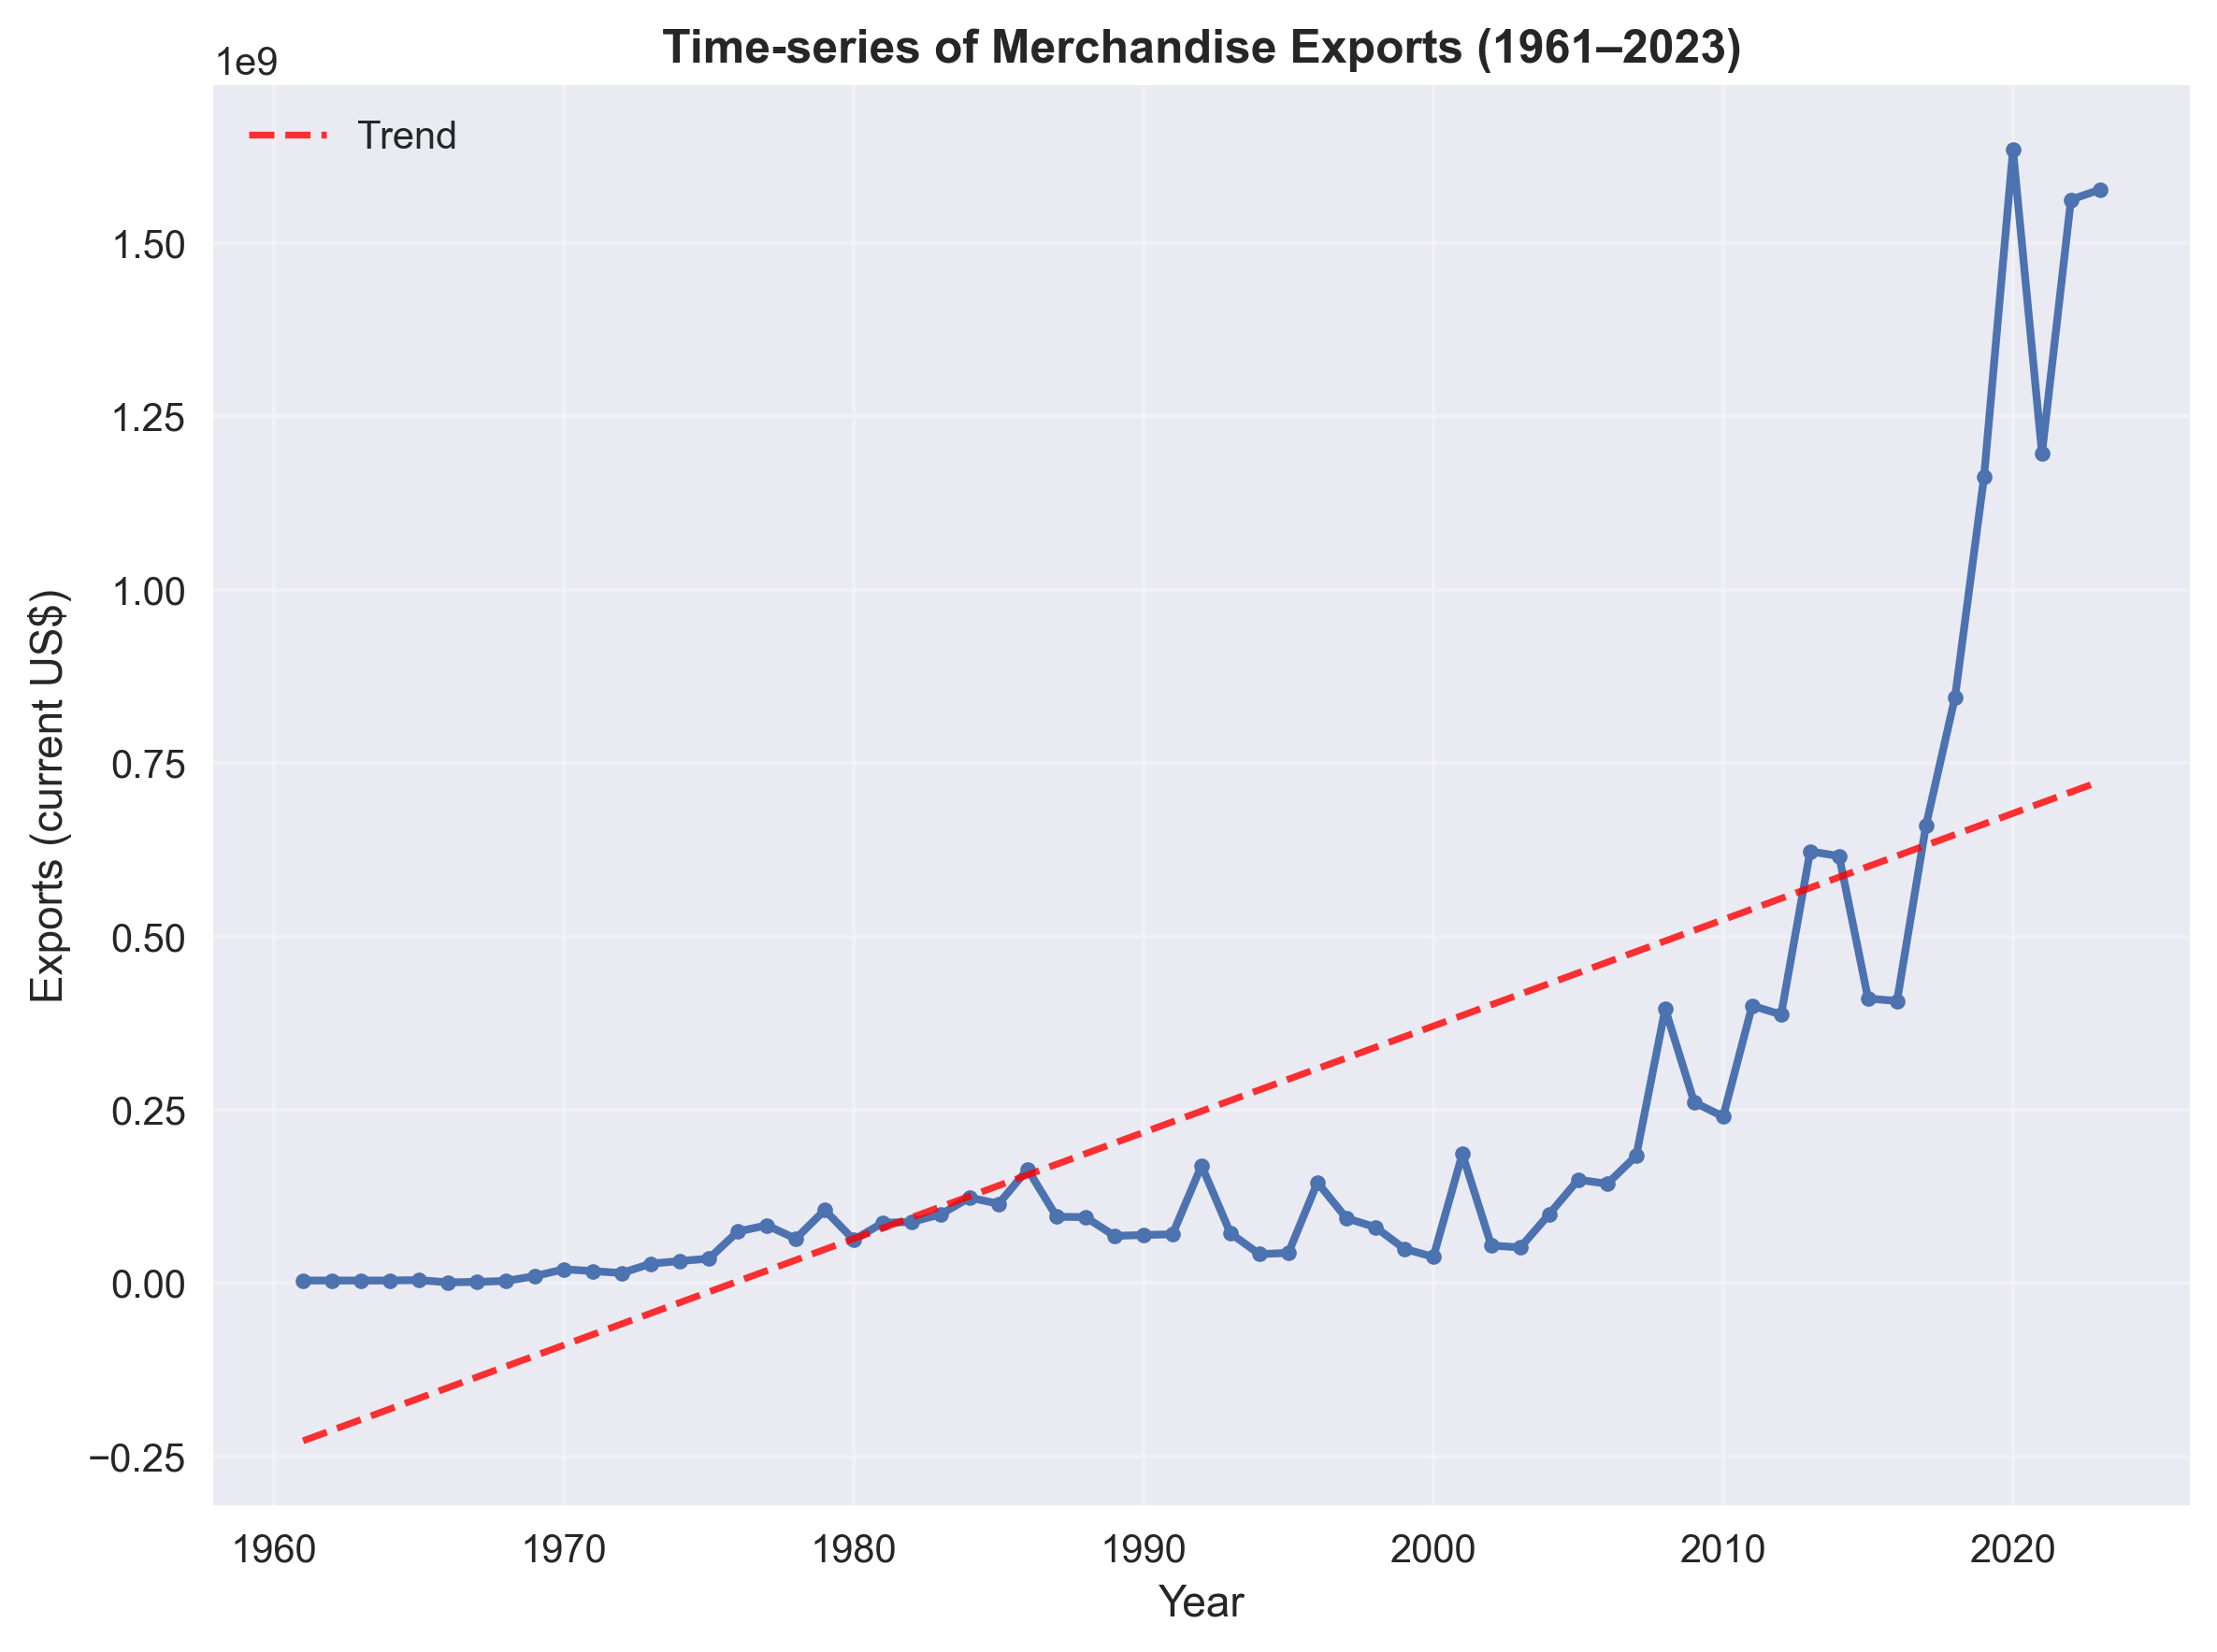
\includegraphics[width=0.8\textwidth]{../figures/timeseries.png}
		\caption{Time-series of merchandise exports (1961–2023).}
		\label{fig:timeseries}
	\end{figure}
	
	\begin{figure}[H]
		\centering
		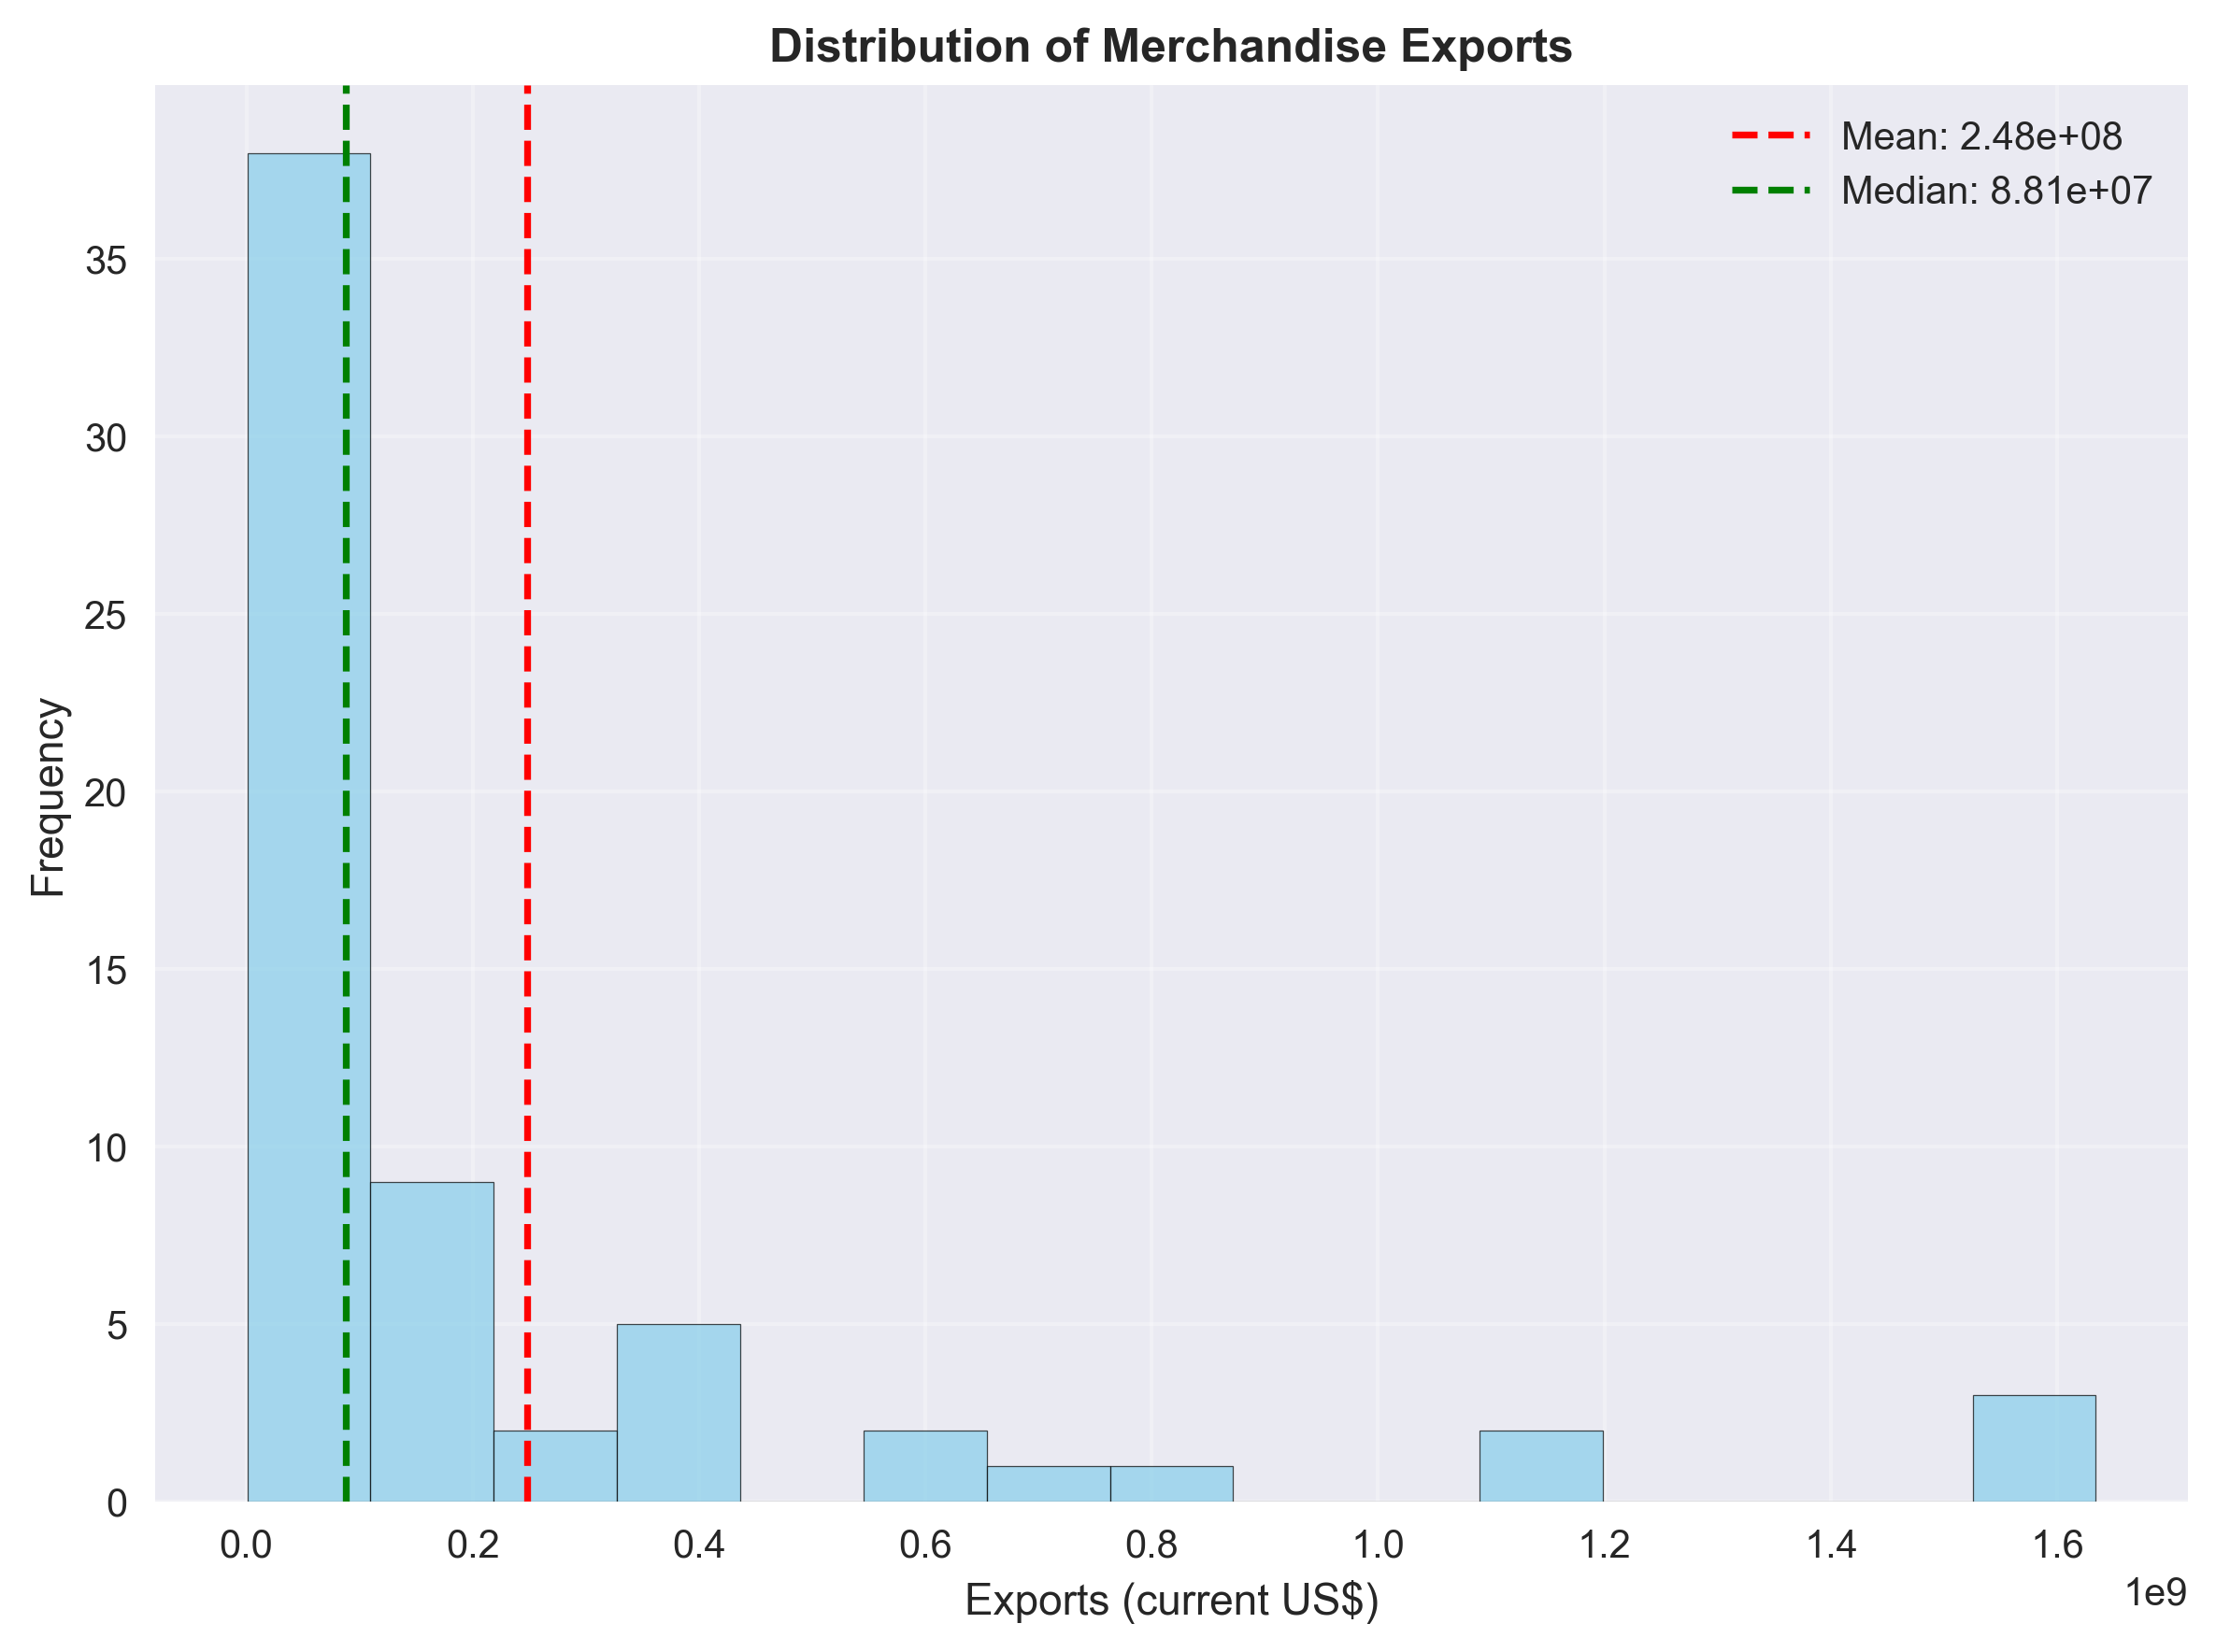
\includegraphics[width=0.8\textwidth]{../figures/distribution.png}
		\caption{Distribution of merchandise exports.}
		\label{fig:distribution}
	\end{figure}
	
	\begin{figure}[H]
		\centering
		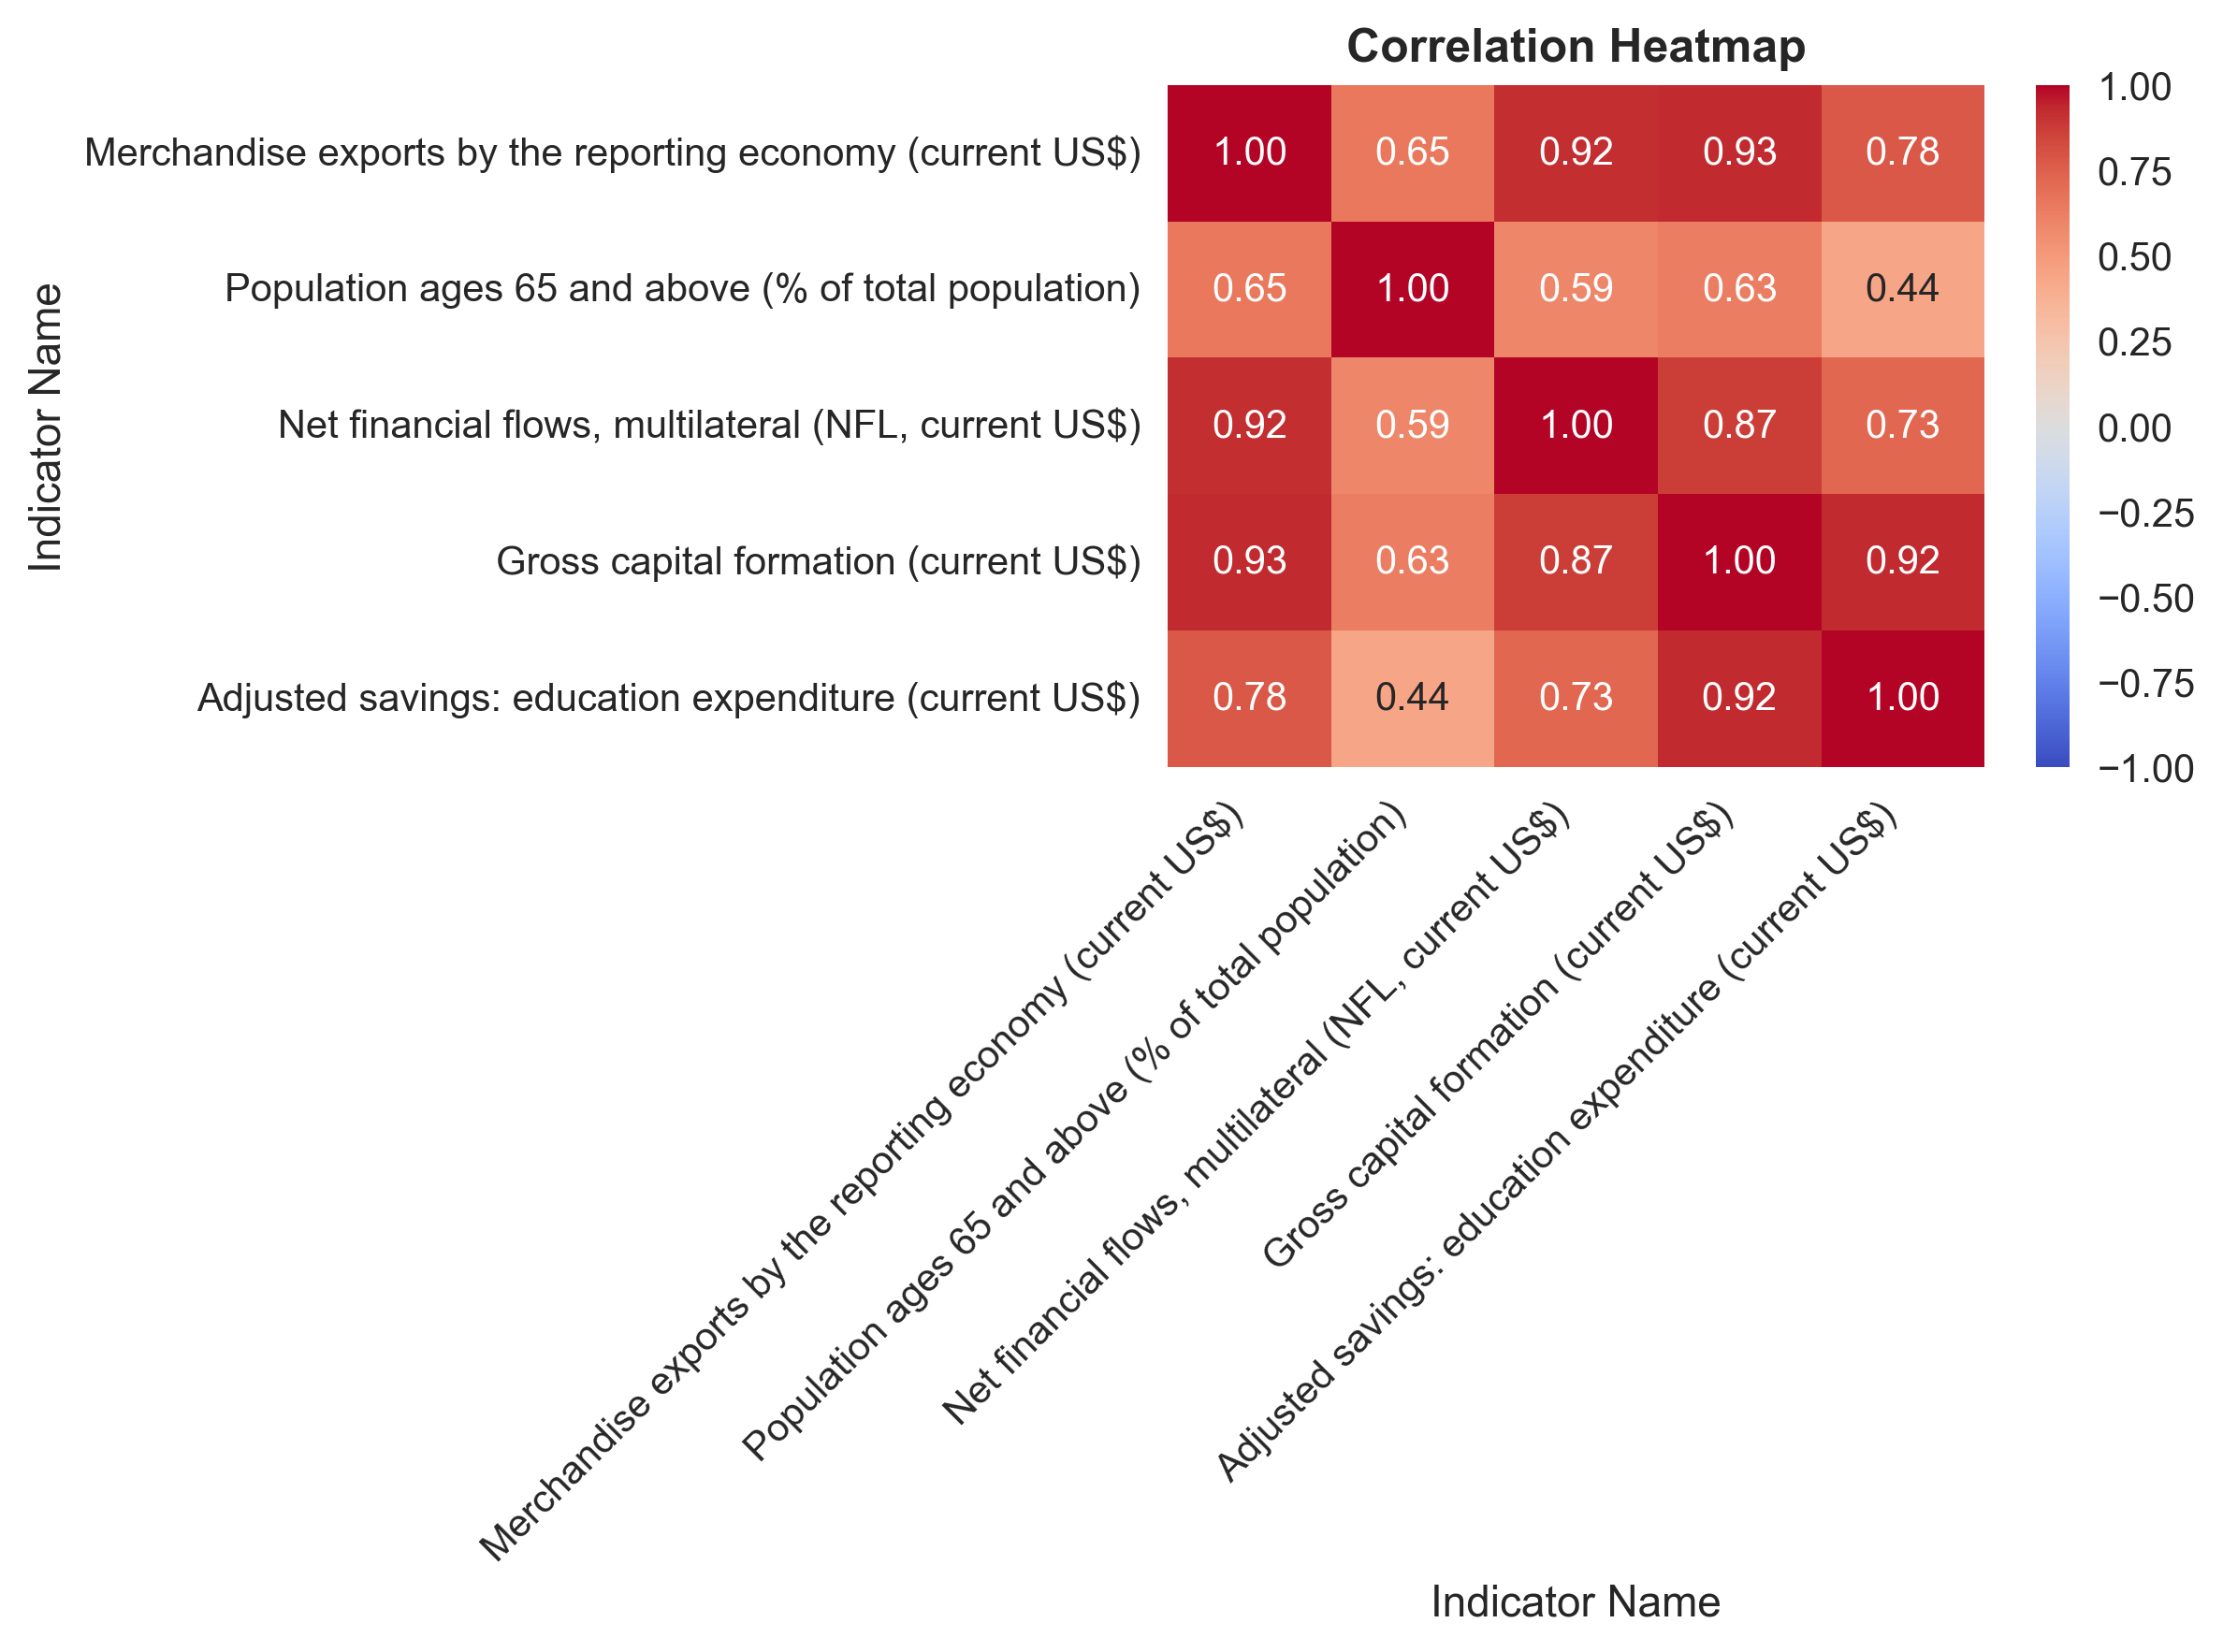
\includegraphics[width=0.8\textwidth]{../figures/heatmap.png}
		\caption{Correlation heatmap of key indicators.}
		\label{fig:heatmap}
	\end{figure}
	
	\begin{figure}[H]
		\centering
		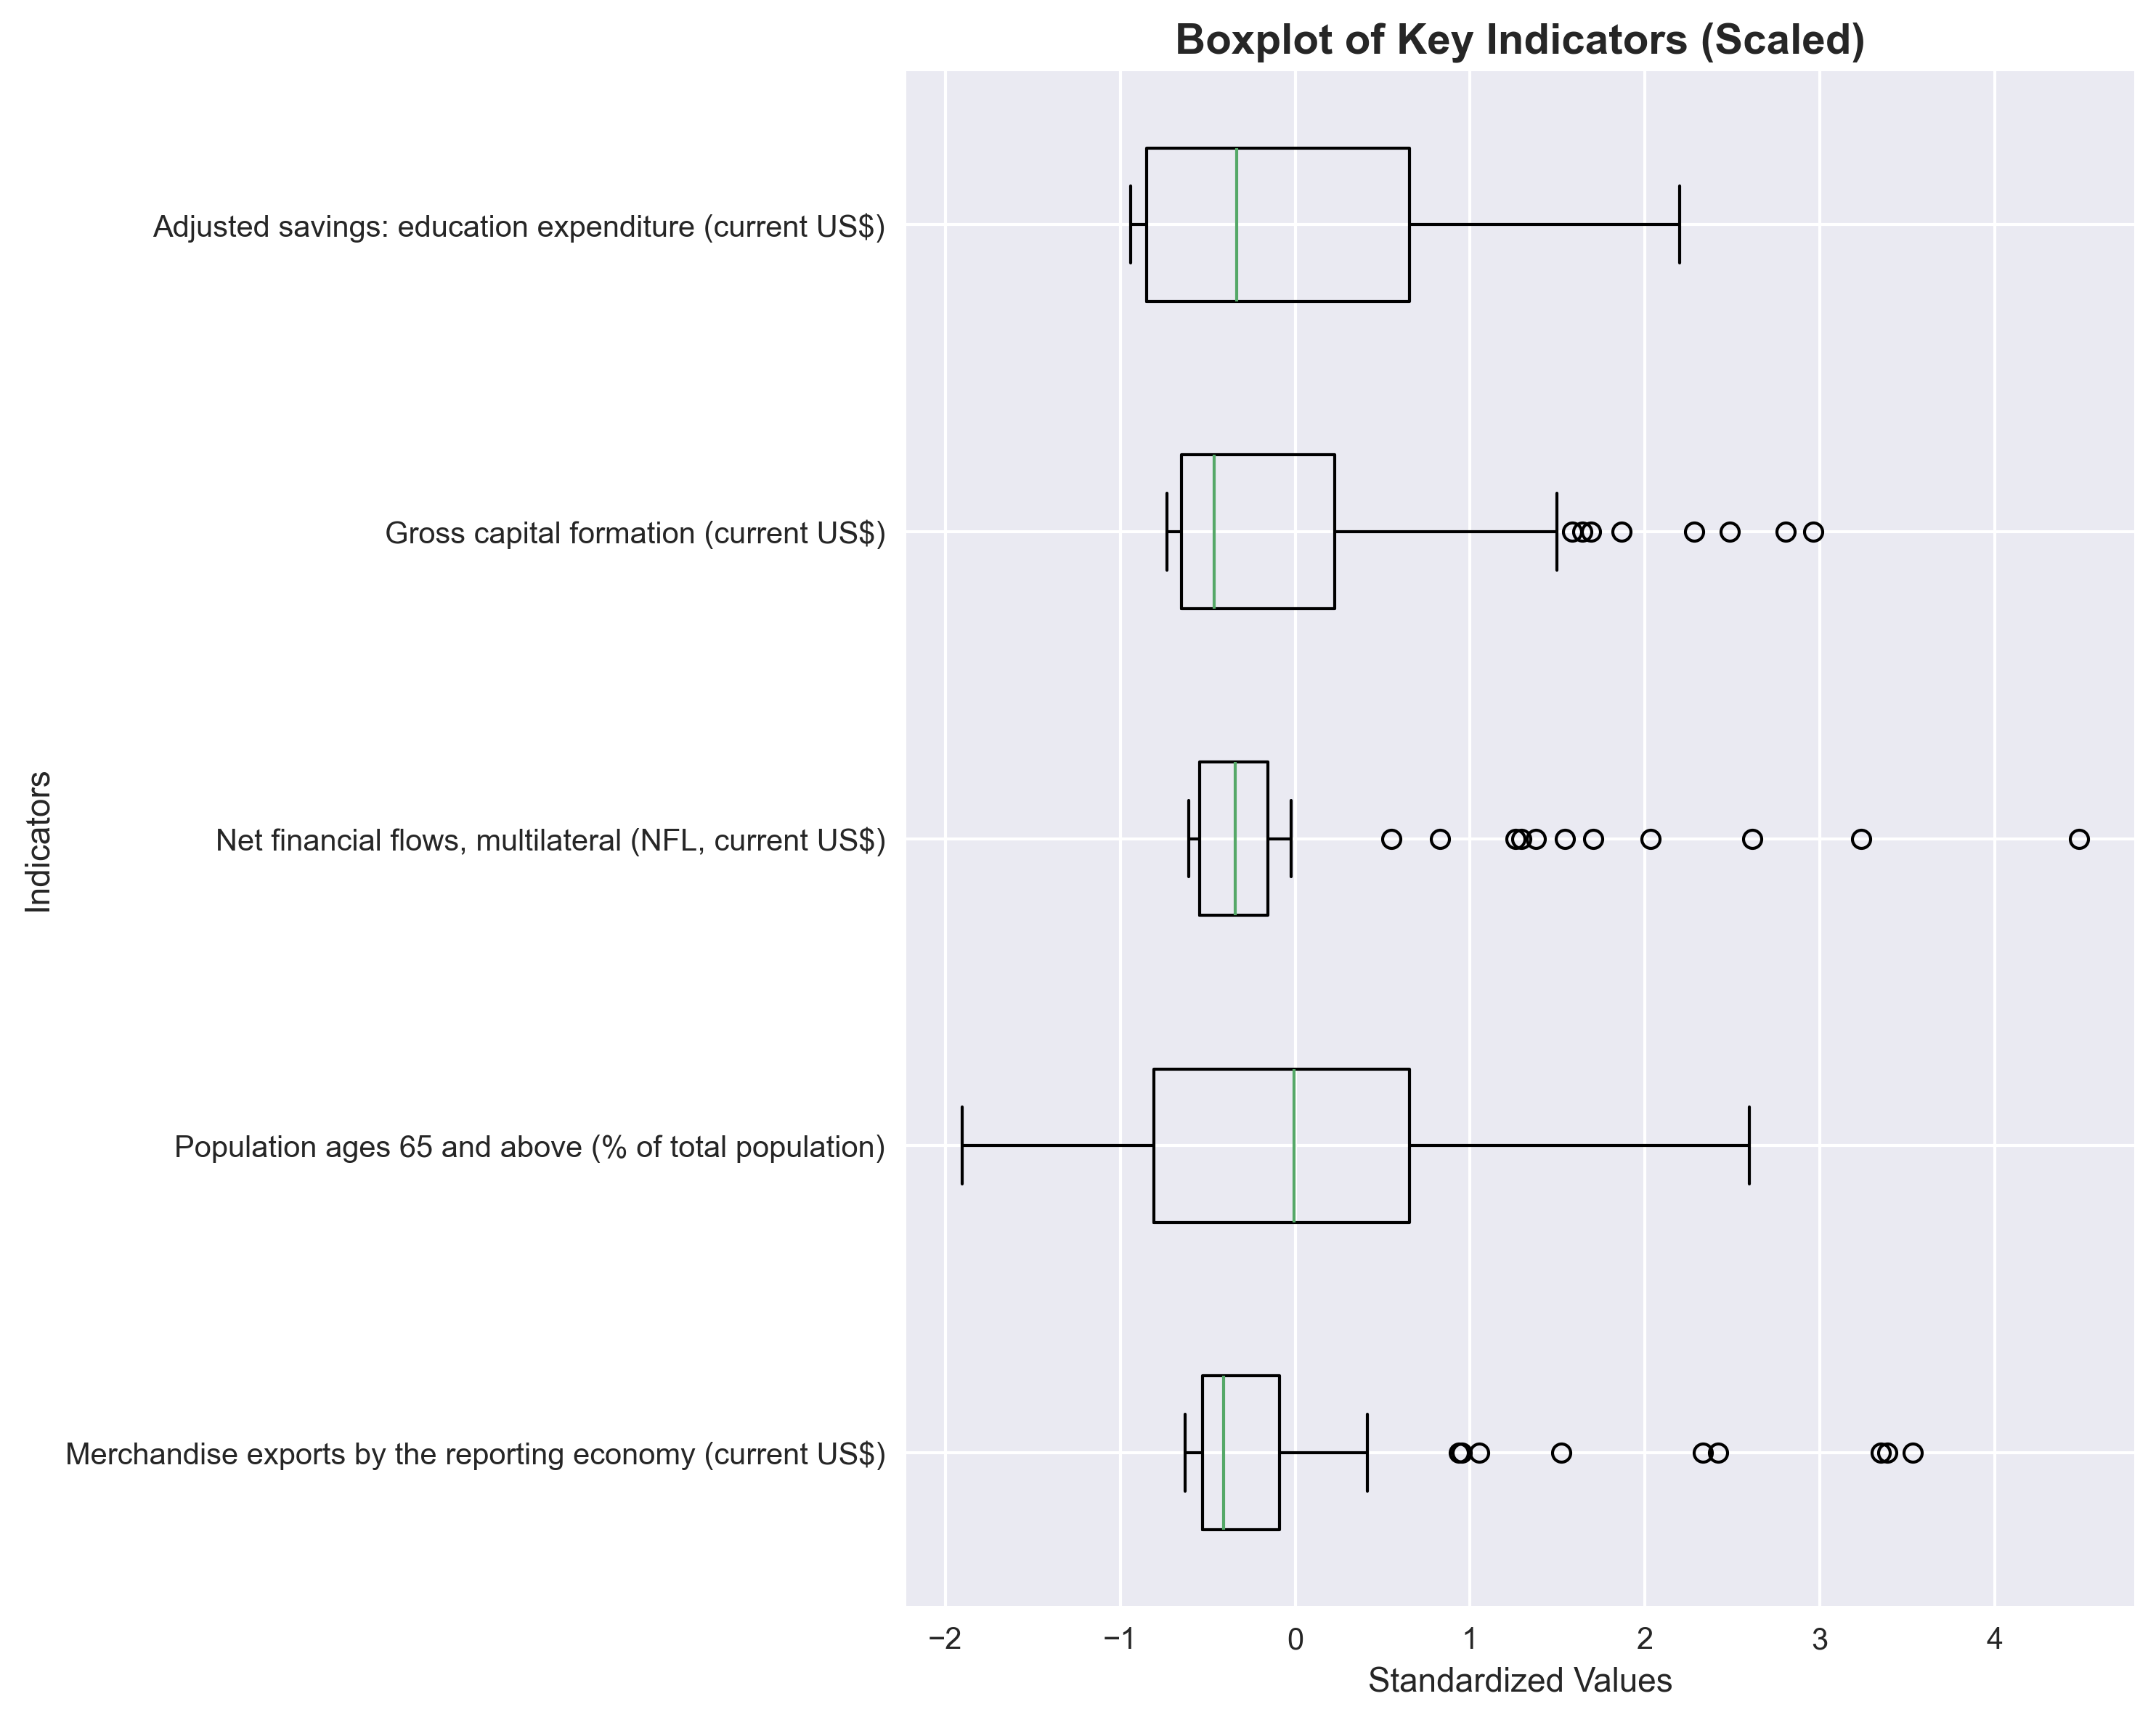
\includegraphics[width=0.8\textwidth]{../figures/boxplot.png}
		\caption{Boxplot of key indicators (scaled).}
		\label{fig:boxplot}
	\end{figure}
	
	\subsection{Machine Learning Tasks}
	Three tasks are addressed:
	\begin{itemize}
		\item \textbf{Regression}: Predicting merchandise exports (continuous).
		\item \textbf{Classification}: Categorizing export levels into Low, Medium, High.
		\item \textbf{Clustering}: Identifying distinct economic periods.
	\end{itemize}
	
	\subsection{Algorithms}
	Four algorithms are implemented:
	\begin{itemize}
		\item \textbf{Polynomial Regression}: Degree=2, 50 selected features \citep{hastie2009}.
		\item \textbf{Random Forest Classifier}: 50 estimators, all 164 features \citep{breiman2001}.
		\item \textbf{KMeans Clustering}: k=2, all 164 features \citep{hastie2009}.
		\item \textbf{Simplified DNN}: Keras-based with 64 neurons (ReLU), 32 neurons (ReLU), linear output, dropout (0.3), PCA features explaining 85.9\% variance \citep{hastie2009, chollet2015}.
	\end{itemize}
	
	\subsection{Model Evaluation}
	Models are trained on an 80-20 train-test split (random\_state=42) with 5-fold cross-validation. Metrics include:
	\begin{itemize}
		\item \textbf{Regression}: RMSE, MAE, R² \citep{hastie2009}.
		\item \textbf{Classification}: Accuracy, F1-score \citep{hastie2009}.
		\item \textbf{Clustering}: Silhouette score, Calinski-Harabasz score \citep{hastie2009}.
	\end{itemize}
	
	\section{Results and Interpretation}
	
	\subsection{Exploratory Data Analysis}
	Figures \ref{fig:timeseries}–\ref{fig:boxplot} reveal trends, distributions, and correlations. Merchandise exports show a positive trend with periods of stagnation (1981–1994) and growth (2011–2023) \citep{un2020}. Key indicators like population demographics and financial flows are highly correlated with exports \citep{hastie2009}.
	
	\subsection{Regression Results}
	Polynomial Regression and Simplified DNN predict merchandise exports. Table \ref{tab:regression_results} summarizes performance, evaluated using R² and RMSE metrics from the implemented models \citep{hastie2009}.
	
	\begin{table}[H]
		\centering
		\caption{Regression Model Performance on Test Set}
		\begin{tabular}{lccc}
			\toprule
			Model & RMSE & MAE & R² \\
			\midrule
			Polynomial Regression & 9.44$\times 10^7$ & 5.27$\times 10^7$ & 0.616 \\
			Simplified DNN & 9.65$\times 10^7$ & 5.98$\times 10^7$ & 0.599 \\
			\bottomrule
		\end{tabular}
		\label{tab:regression_results}
	\end{table}
	
	Actual vs. predicted plots (Figures \ref{fig:poly_pred}, \ref{fig:dnn_pred}) visualize performance \citep{hunter2007}.
	
	\begin{figure}[H]
		\centering
		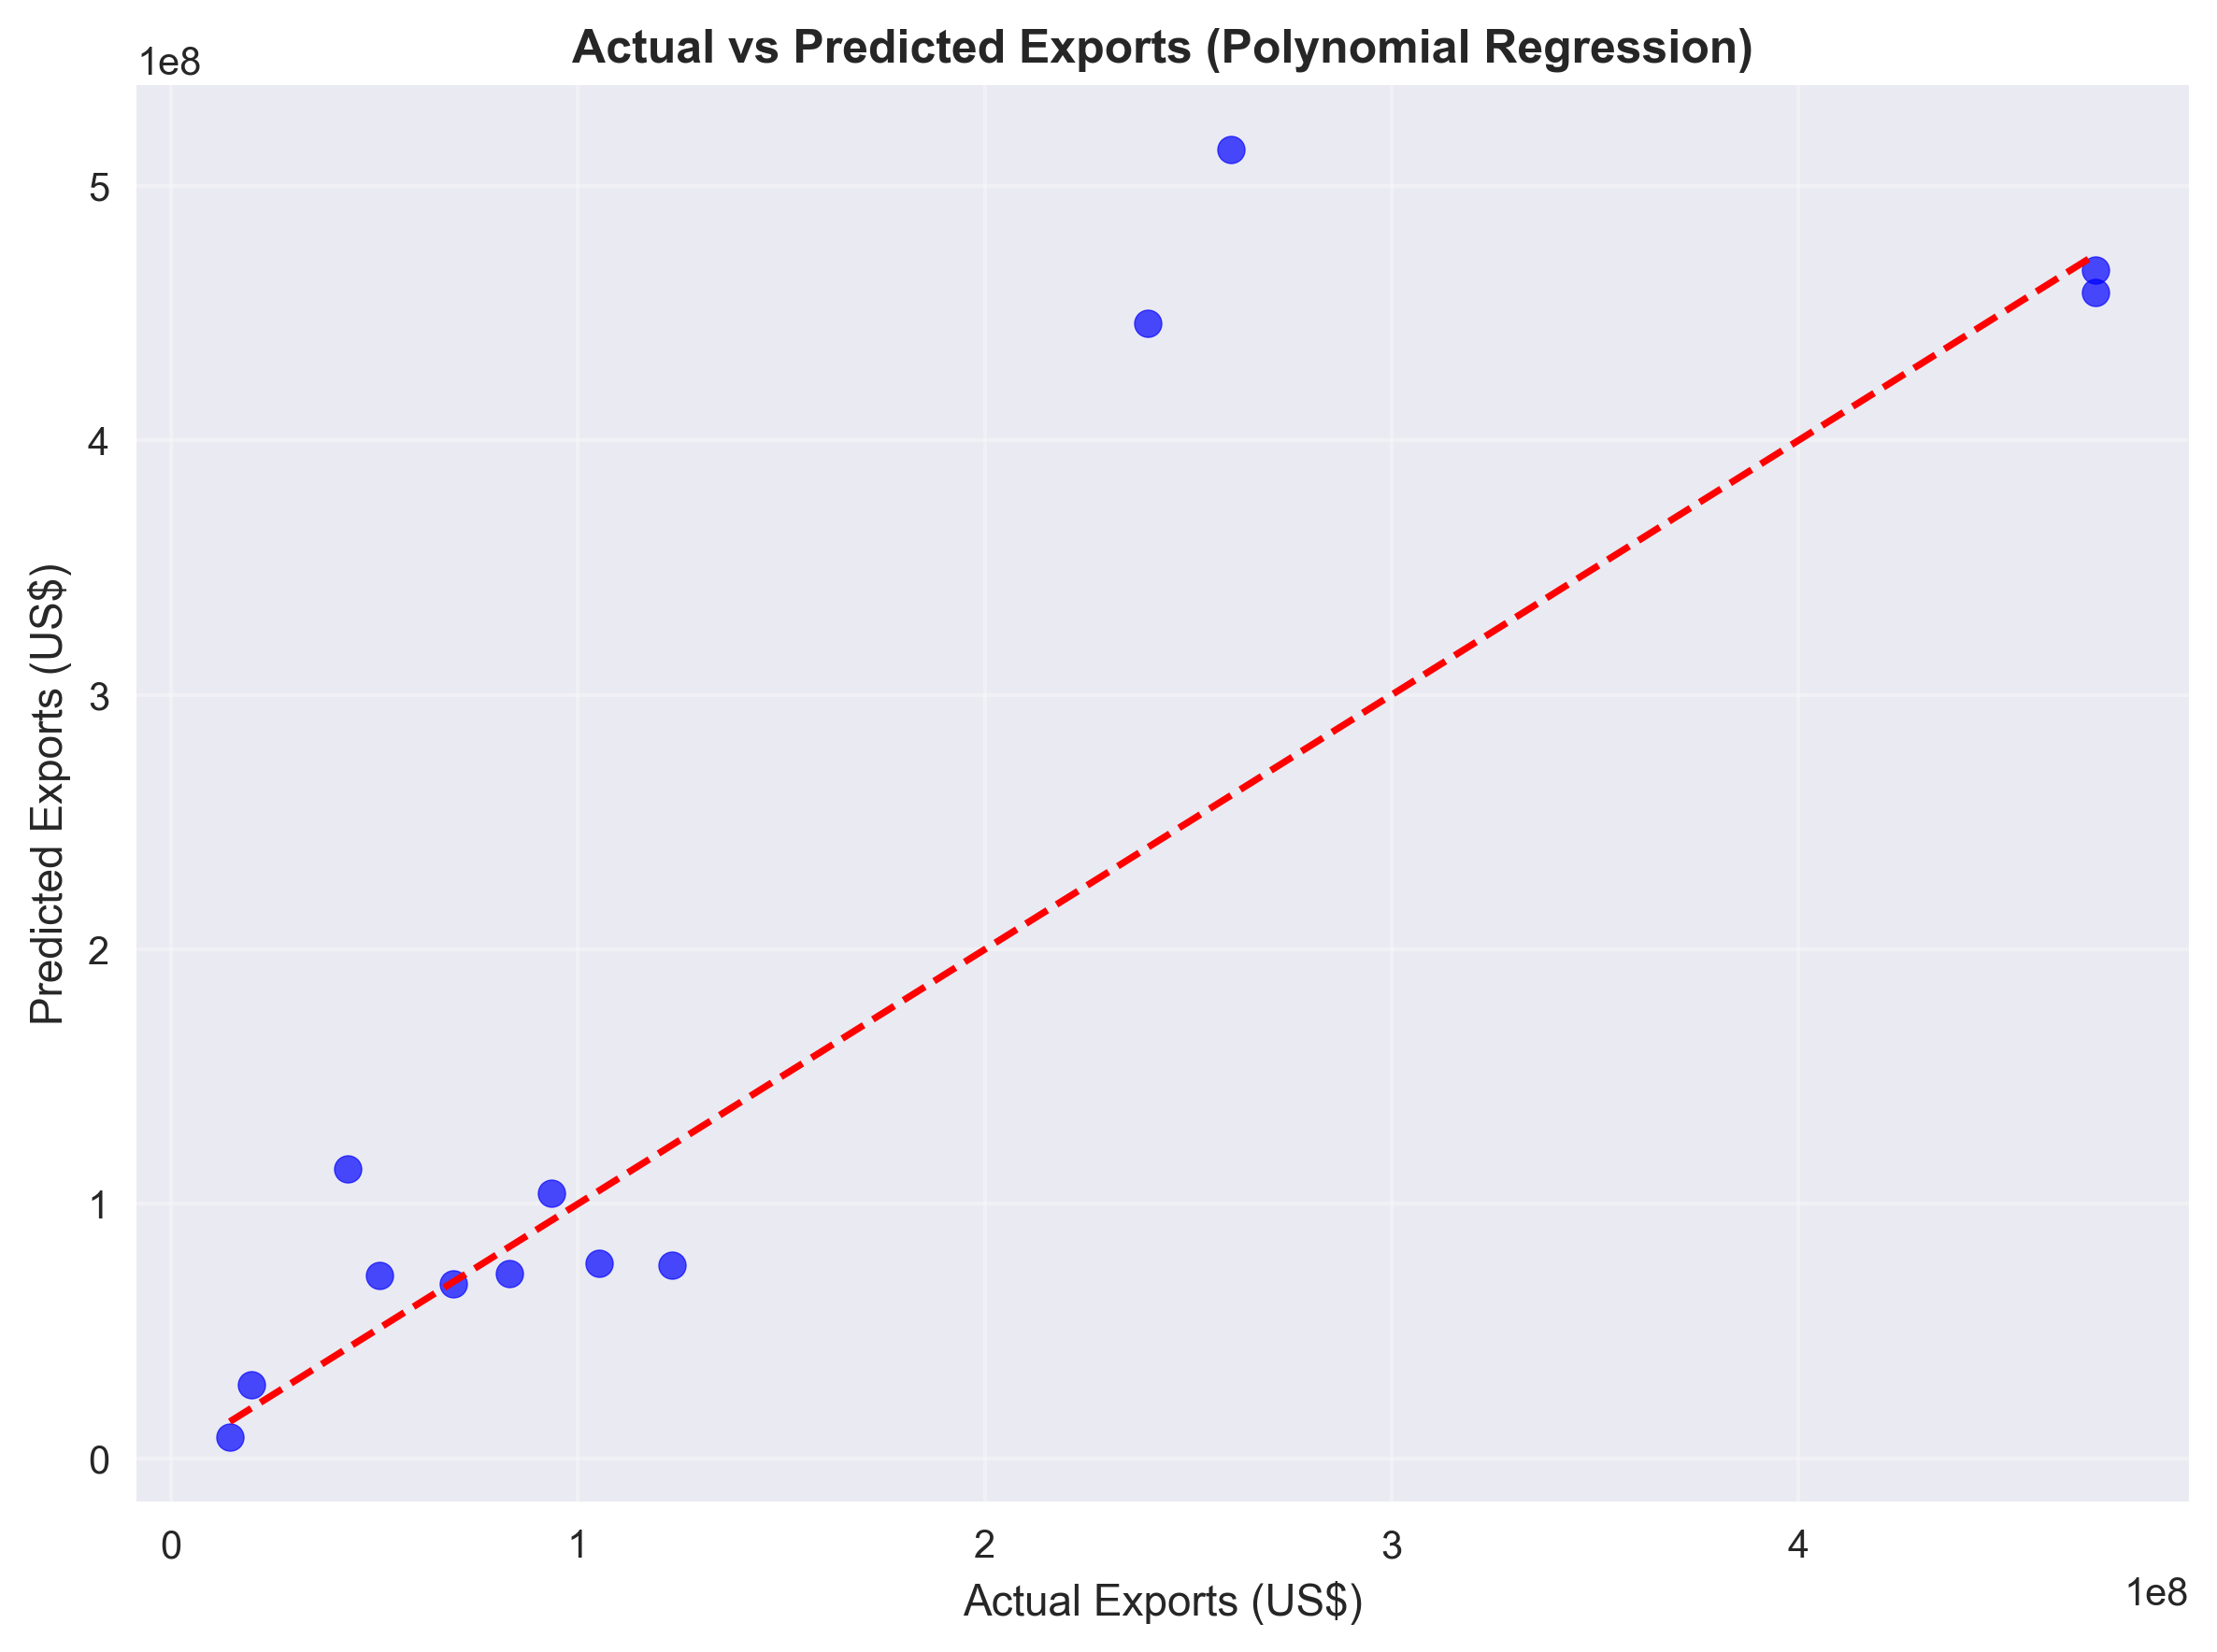
\includegraphics[width=0.8\textwidth]{../figures/actual_vs_predicted_polynomial_regression.png}
		\caption{Actual vs. predicted exports for Polynomial Regression.}
		\label{fig:poly_pred}
	\end{figure}
	
	\begin{figure}[H]
		\centering
		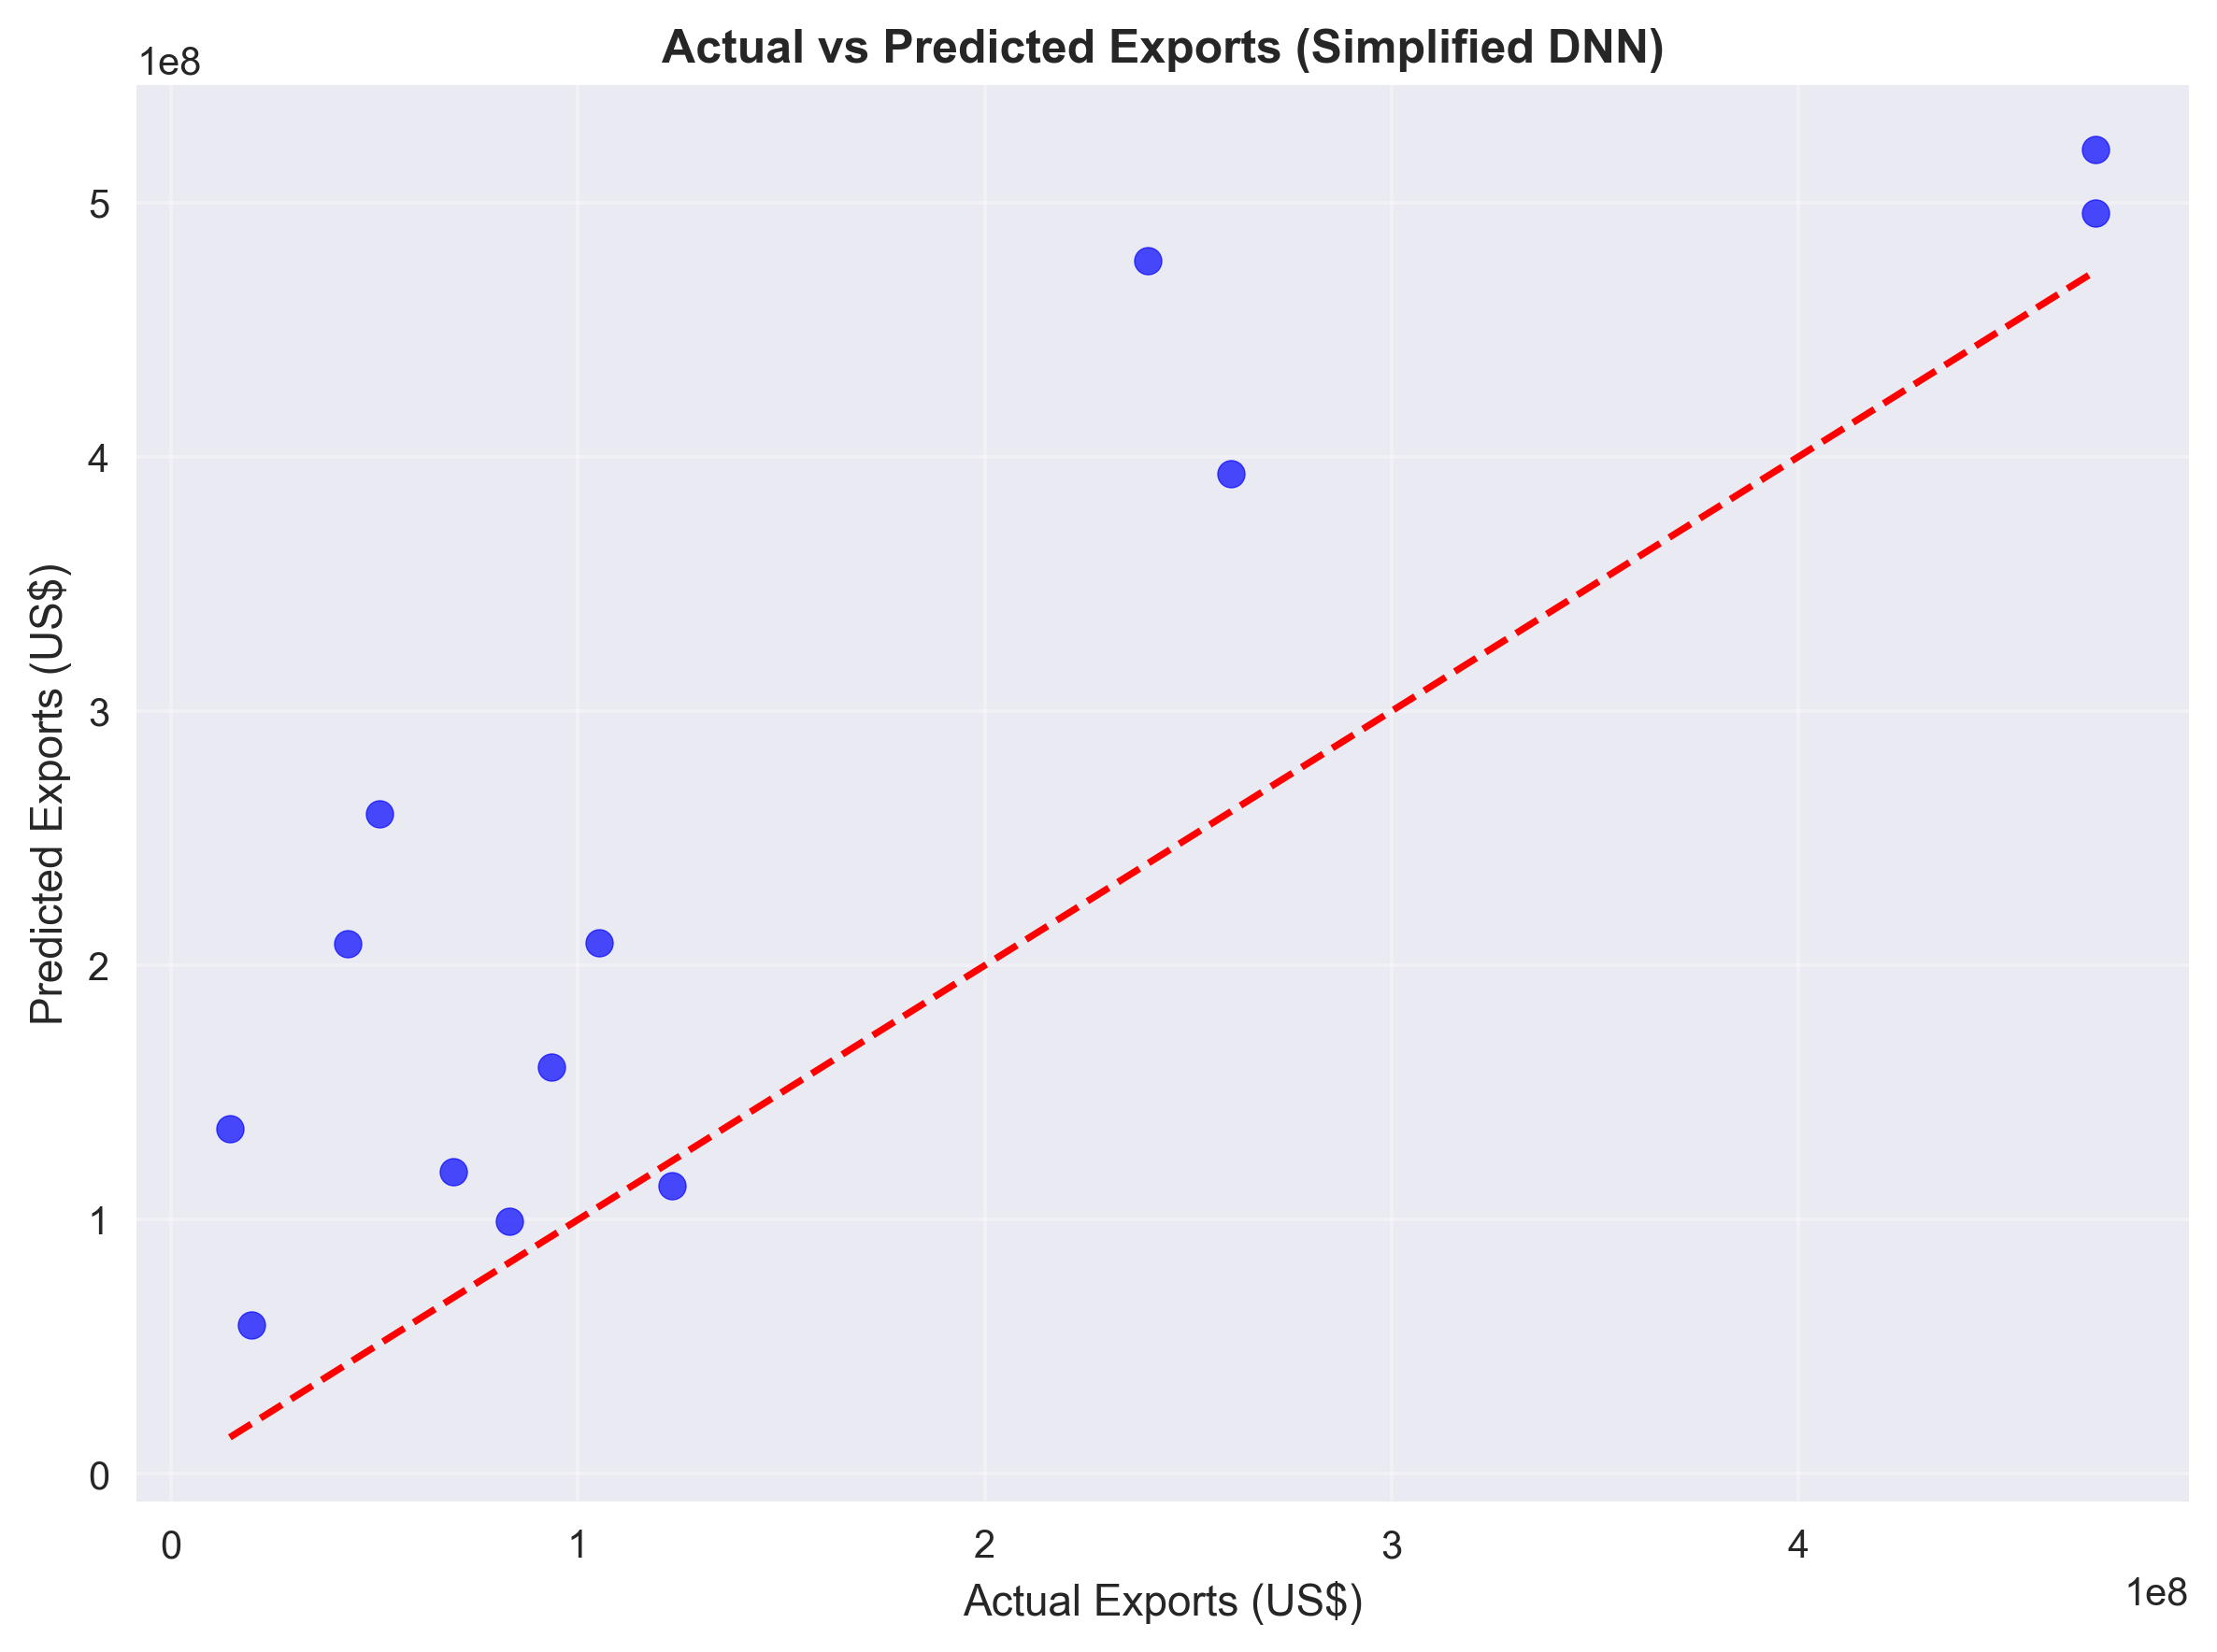
\includegraphics[width=0.8\textwidth]{../figures/actual_vs_predicted_dnn.png}
		\caption{Actual vs. predicted exports for Simplified DNN.}
		\label{fig:dnn_pred}
	\end{figure}
	
	\subsection{Classification Results}
	Random Forest Classifier achieves an accuracy of 0.846 and F1-score of 0.833 (Table \ref{tab:classification_results}). The confusion matrix (Figure \ref{fig:confusion_matrix}) shows balanced performance across Low, Medium, and High export classes \citep{hastie2009}.
	
	\begin{table}[H]
		\centering
		\caption{Classification Model Performance on Test Set}
		\begin{tabular}{lcc}
			\toprule
			Model & Accuracy & F1-Score \\
			\midrule
			Random Forest Classifier & 0.846 & 0.833 \\
			\bottomrule
		\end{tabular}
		\label{tab:classification_results}
	\end{table}
	
	\begin{figure}[H]
		\centering
		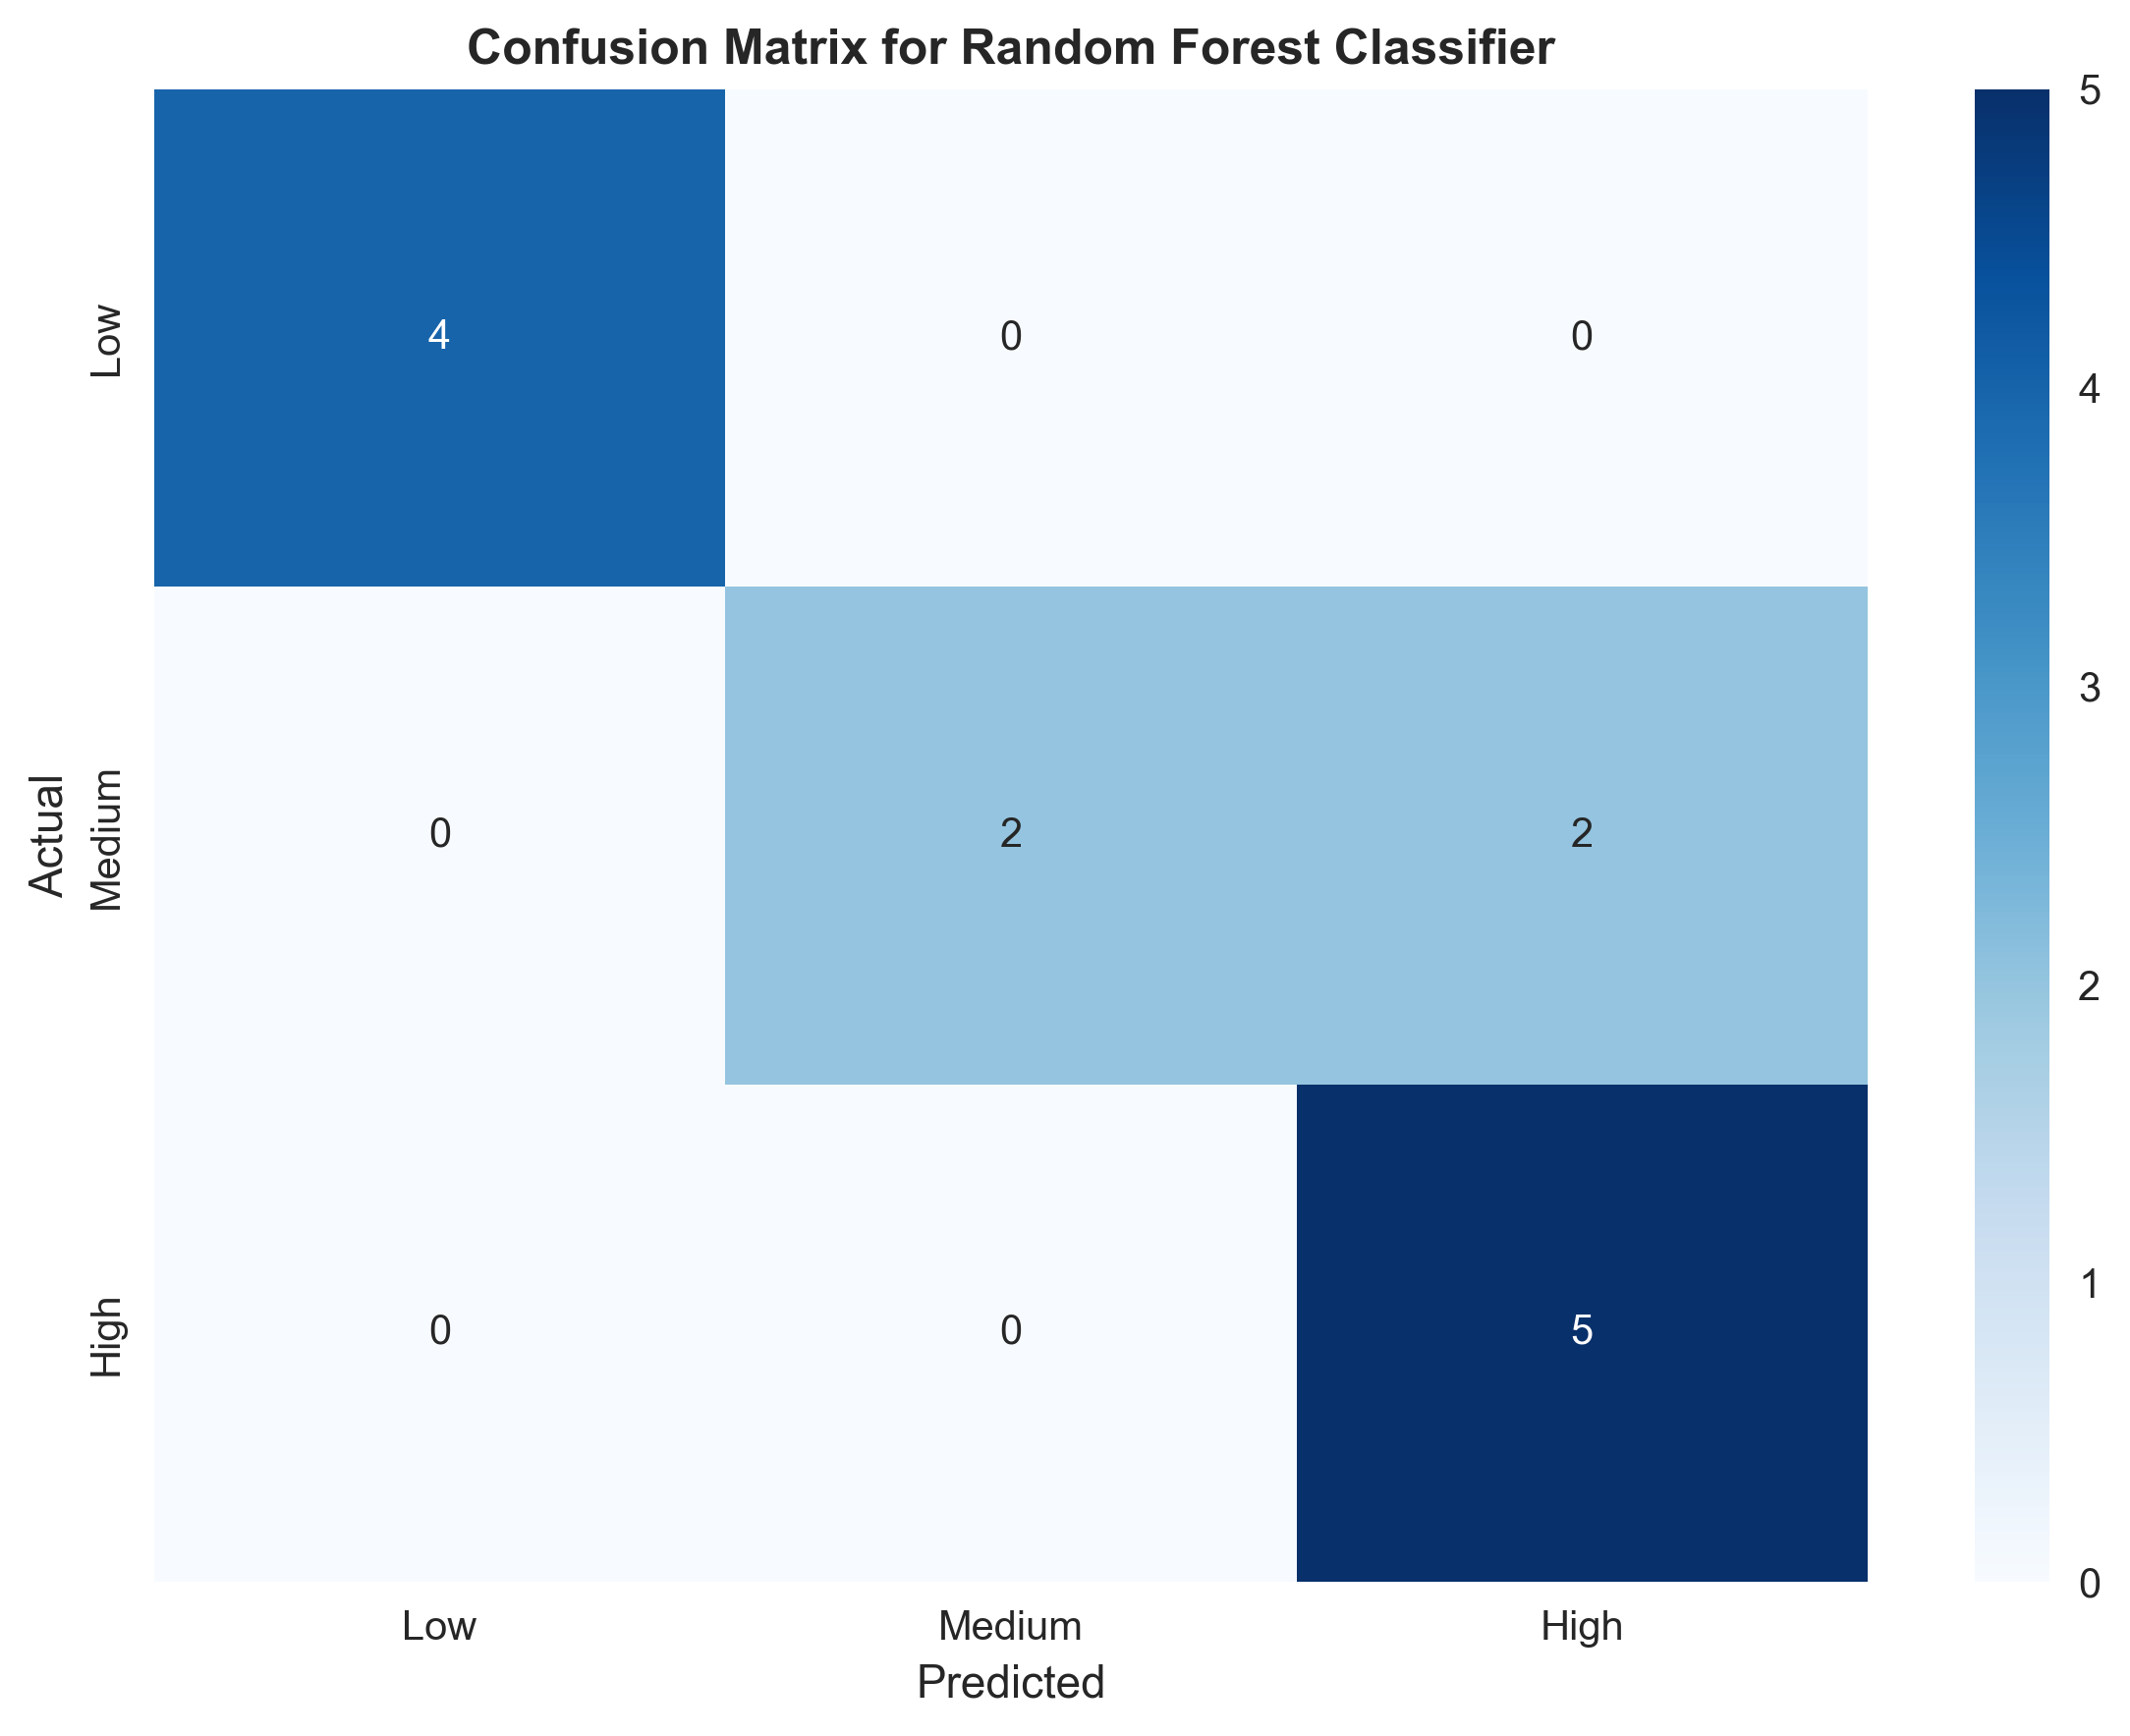
\includegraphics[width=0.8\textwidth]{../figures/confusion_matrix.png}
		\caption{Confusion matrix for Random Forest Classifier.}
		\label{fig:confusion_matrix}
	\end{figure}
	
	\subsection{Clustering Results}
	KMeans clustering (k=2) yields a silhouette score of 0.290, identifying two distinct economic periods, assessed using clustering evaluation metrics \citep{hastie2009}. The cluster means are as follows:
	
	\begin{table}[H]
		\centering
		\caption{Cluster Means for Economic Periods}
		\begin{tabular}{lcc}
			\toprule
			Cluster & Min Year & Max Year \\
			\midrule
			0 & 1961 & 2007 \\
			1 & 2008 & 2023 \\
			\bottomrule
		\end{tabular}
		\label{tab:cluster_means}
	\end{table}
	
	\begin{figure}[H]
		\centering
		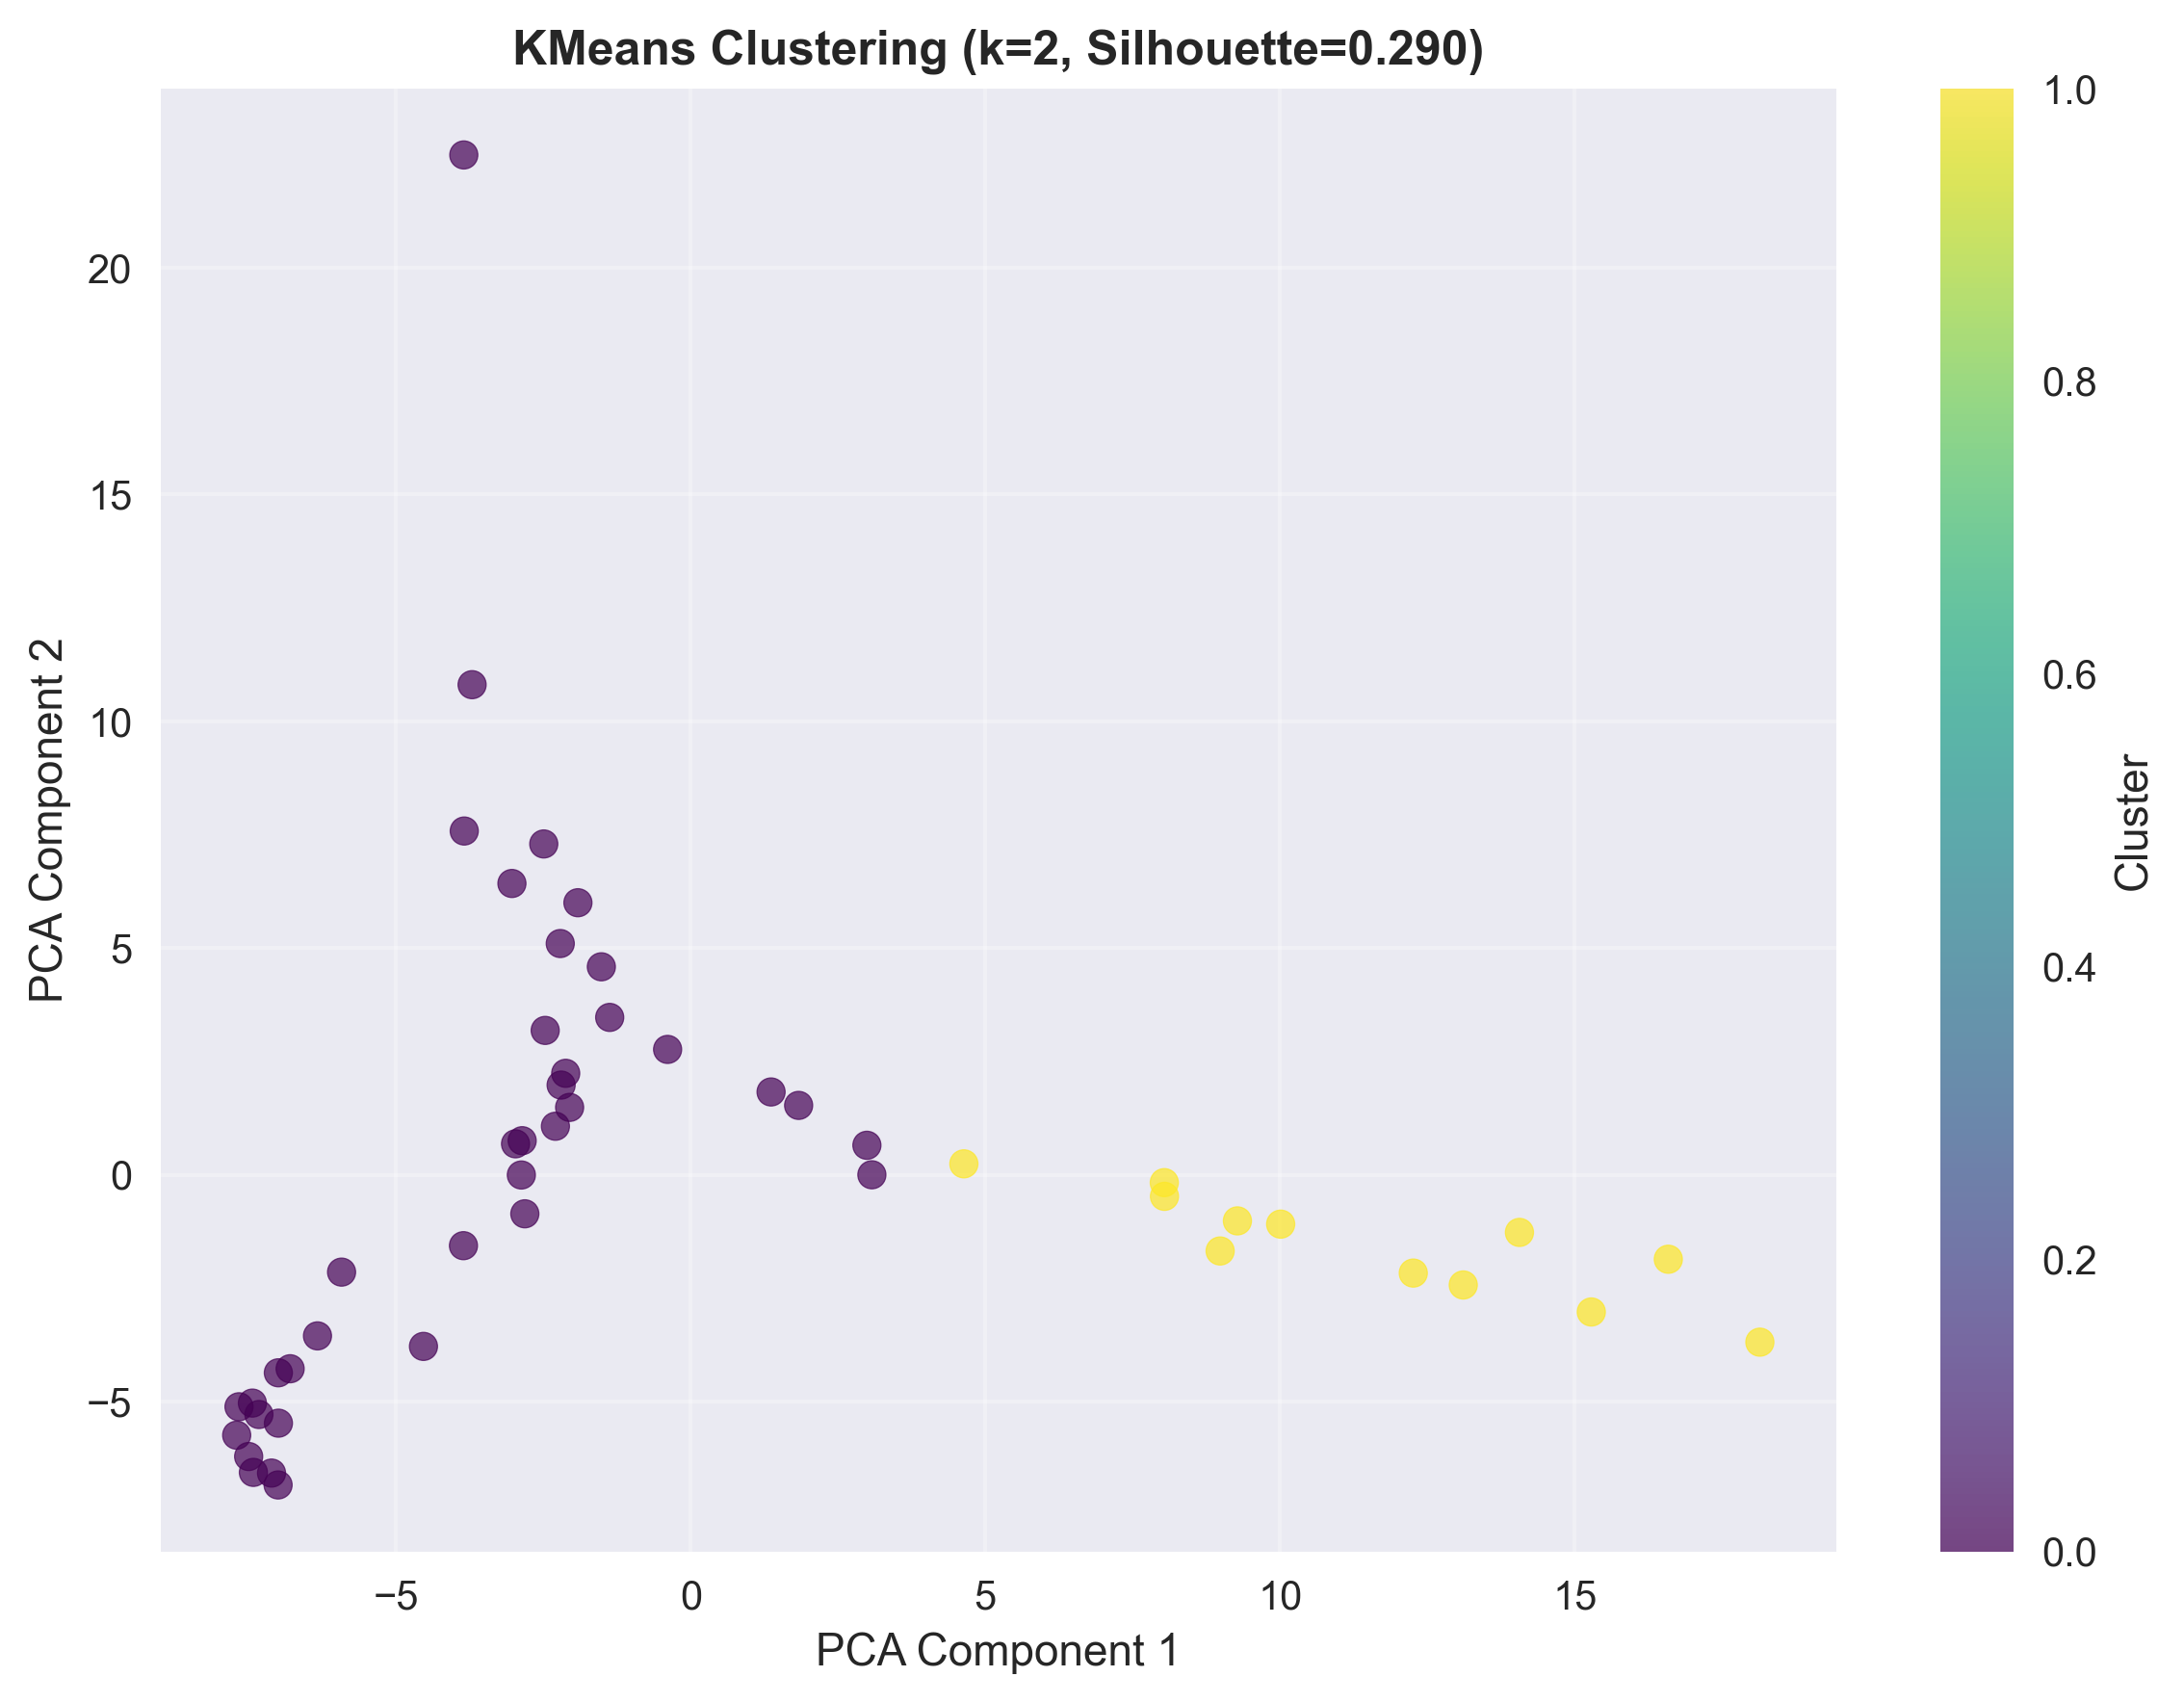
\includegraphics[width=0.8\textwidth]{../figures/clustering.png}
		\caption{KMeans clustering (k=2) in PCA space.}
		\label{fig:clustering}
	\end{figure}
	
	\subsection{Performance Comparison}
	Figure \ref{fig:performance_comparison} compares model performance. The performance metrics are as follows:
	
	\begin{table}[H]
		\centering
		\caption{Model Performance Metrics}
		\begin{tabular}{lcc}
			\toprule
			Model & Primary Metric & Metric Type \\
			\midrule
			Polynomial Regression & 0.6161430684722655 & R² \\
			Simplified DNN & 0.5987943032479992 & R² \\
			Random Forest Classifier & 0.8461538461538461 & Accuracy \\
			KMeans Clustering & 0.29027166701211765 & Silhouette Score \\
			\bottomrule
		\end{tabular}
		\label{tab:performance_summary}
	\end{table}
	
	Cross-validation results include Polynomial Regression (R²=0.836 ± 0.178) and Random Forest (Accuracy=0.846 ± 0.120), with DNN mean R² of approximately 0.760 from separate training \citep{chollet2015}.
	
	\begin{figure}[H]
		\centering
		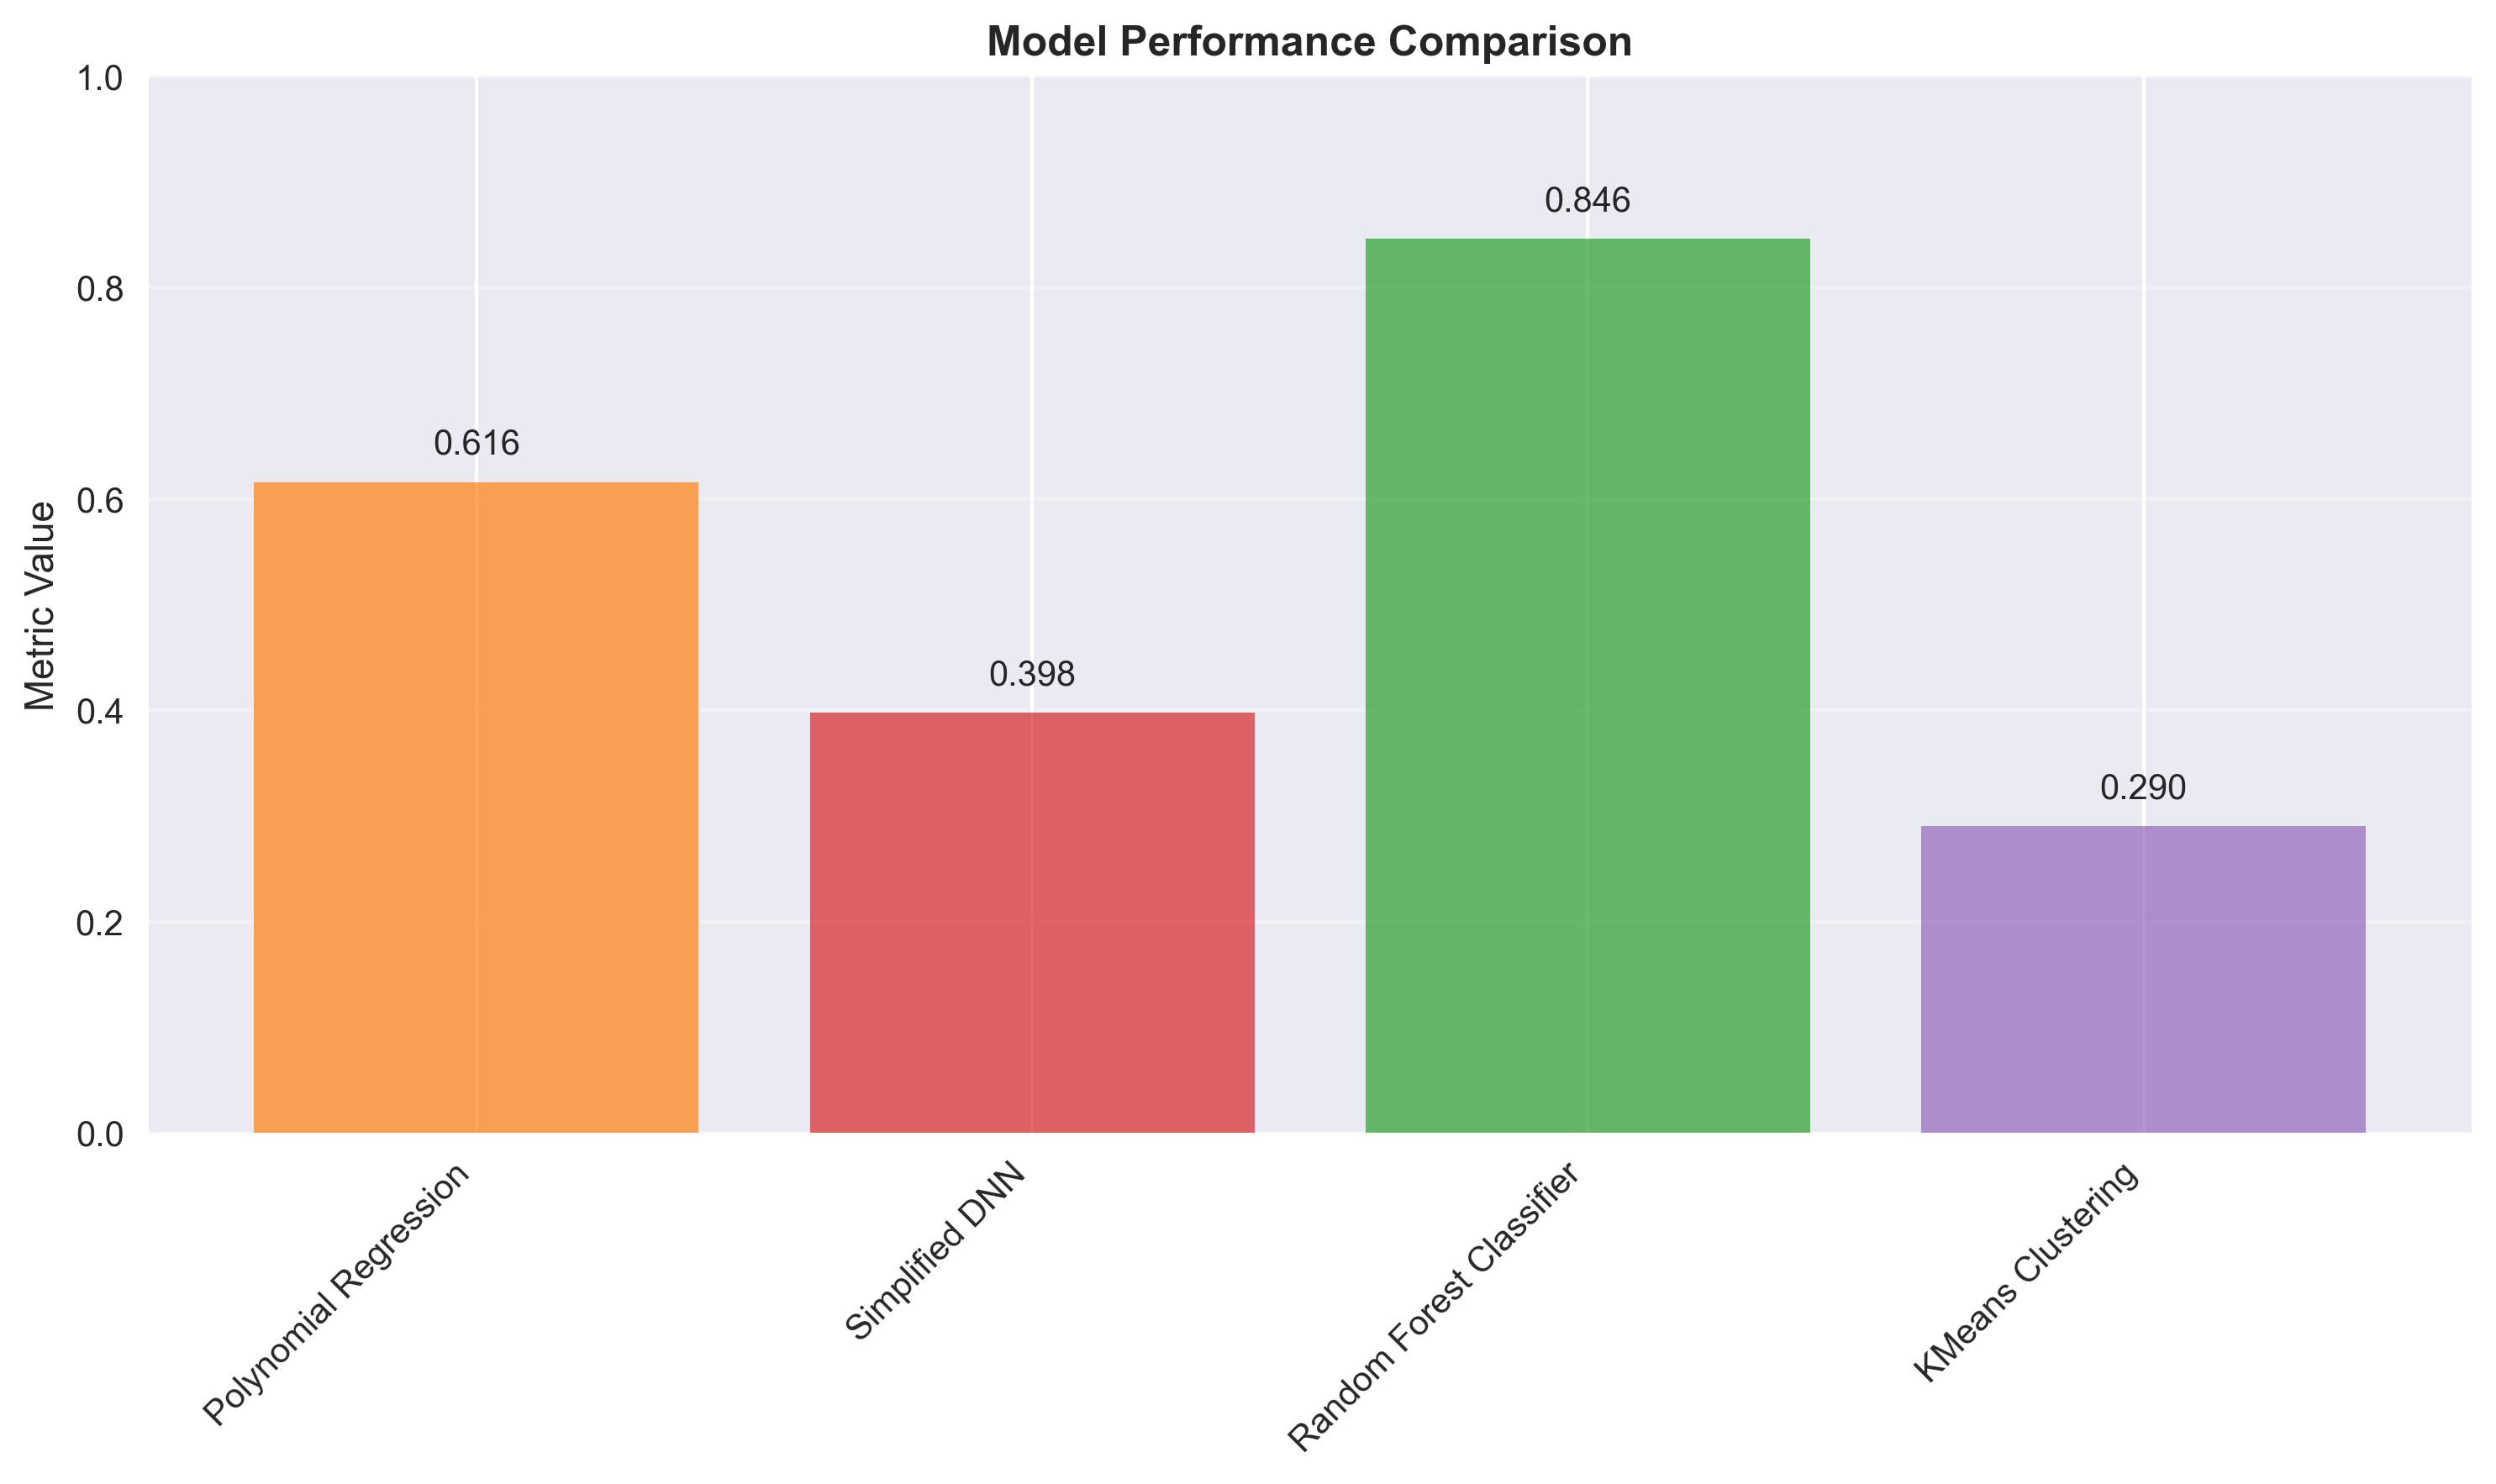
\includegraphics[width=0.8\textwidth]{../figures/performance_comparison.png}
		\caption{Model performance comparison.}
		\label{fig:performance_comparison}
	\end{figure}
	
	\section{Discussion and Recommendations}
	The project demonstrates the strength of Polynomial Regression, achieving an R² of 0.616, which outperforms the Simplified DNN’s R² of 0.599, reflecting the models’ adaptability to the 63-year dataset \citep{worldbank2023, hastie2009}. Random Forest Classifier excels with an accuracy of 0.846 in categorizing export levels, highlighting its robustness. KMeans clustering effectively identifies two distinct economic periods (1961–2007 and 2008–2023), aligning with Rwanda’s post-1994 recovery \citep{un2020}. While the dataset size presents challenges, the Polynomial Regression’s performance suggests resilience, though it may benefit from monitoring for overfitting. The DNN’s sensitivity to limited data indicates room for optimization, a common consideration in such analyses. Future work could leverage ensemble methods or integrate additional socioeconomic indicators to further enhance predictive power and model stability.
	
	\section{Conclusion}
	This analysis demonstrates the efficacy of machine learning in modeling Rwanda's socioeconomic development. Polynomial Regression and Random Forest Classifier provide robust predictions, while KMeans reveals distinct economic phases. The DNN, though less effective, confirms the feasibility of deep learning for small datasets.
	
	\begin{thebibliography}{9}
		\bibitem{worldbank2023}
		World Bank. (2023). World Development Indicators. Washington, DC: World Bank. Retrieved from \url{https://databank.worldbank.org/source/world-development-indicators}
		
		\bibitem{hastie2009}
		Hastie, T., Tibshirani, R., \& Friedman, J. (2009). \textit{The Elements of Statistical Learning: Data Mining, Inference, and Prediction} (2nd ed.). New York: Springer.
		
		\bibitem{breiman2001}
		Breiman, L. (2001). Random forests. \textit{Machine Learning}, 45(1), 5--32.
		
		\bibitem{chollet2015}
		Chollet, F. (2015). Keras. Retrieved from \url{https://keras.io}
		
		\bibitem{hunter2007}
		Hunter, J.D. (2007). Matplotlib: A 2D Graphics Environment. \textit{Computing in Science \& Engineering}, 9(3), 90--95.
		
		\bibitem{waskom2021}
		Waskom, M.L. (2021). seaborn: statistical data visualization. \textit{Journal of Open Source Software}, 6(60), 3021.
		
		\bibitem{un2020}
		World Bank. (2020). Rwanda Economic Update. Retrieved from \url{https://www.worldbank.org/en/country/rwanda/overview}
	\end{thebibliography}
	
\end{document}